\documentclass[a4paper]{article}
\usepackage{fontspec}
\usepackage{ctex}
\usepackage{CJKutf8}
\usepackage{graphicx}
\usepackage{ulem}
\usepackage{ragged2e}
\usepackage{multirow}
\usepackage{color}
\usepackage{array}
\usepackage{indentfirst}
\usepackage{float}
\usepackage{amsmath}
\usepackage{hyperref}

\usepackage{cite}
\bibliographystyle{IEEEtran}

\graphicspath{{figures/}}
\usepackage[left=1.25in,right=1.25in,top=1in,bottom=1in]{geometry}
\pagestyle{empty}

\begin{document}
		\begin{titlepage}
			\centering
			\vspace*{5em}
			\fontsize{26pt}\baselineskip{江西省研究生创新专项资金项目}
			\vspace*{2em}
			
			\fontsize{26pt}\baselineskip{申\hspace{4em} 请\hspace{4em} 表}
			%\textbf{《科研方法论》课程报告}
			\begin{flushleft}
			\vskip 5cm
			\fontsize{14pt}\baselineskip
			\makebox[39mm]{项\qquad 目\qquad 名\qquad 称:}
			%\underline{信息与工程学院学院学学院}
			\underline{\shortstack[l]{\makebox[75mm][c]{基于知识蒸馏的人体姿态估计}}}
			
			%\vskip 0.5cm
			%\makebox[39mm]{}
			%\underline{\makebox[75mm][c]{信息与工程学院学院学学院}}
			
			\vskip 0.9cm
			\makebox[40mm]{申\hspace{1.4cm}请\hspace{1.4cm}人:}
			\underline{\makebox[75mm][c]{谢唯嘉}}\\
			
			\vskip 0.9cm
			\makebox[39mm]{指\qquad 导\qquad 教\qquad 师:}
			\underline{\makebox[75mm][c]{易见兵 \qquad 副教授}}\\
			
			\vskip 0.9cm
			\makebox[39mm]{培\hspace{0.2cm}养\hspace{0.2cm}单\hspace{0.2cm}位(盖\quad 章):}
			\underline{\makebox[75mm][c]{江西理工大学}}\\
			
			\vskip 0.9cm
			\makebox[40mm]{填\qquad 报\qquad 时\qquad 间:}
			\underline{\makebox[75mm][c]{\today}}
			\vskip 2cm
			
			\end{flushleft}
					 
		\end{titlepage}
\newpage

\begin{table}[H]
	\centering
	\renewcommand\arraystretch{1.7}
	\begin{tabular}{|c|c|c|c|c|} 
		\hline
		\multicolumn{5}{|l|}{一\textcolor[rgb]{0.2,0.2,0.2}{\textbf{、项目申报人基本情况}}}                                             \\ 
		\hline
		\begin{tabular}[c]{@{}c@{}}姓名\\ \end{tabular}          & 谢唯嘉         & 性别     & 男       & \multirow{4}{*}{\begin{minipage}{0.2\columnwidth}{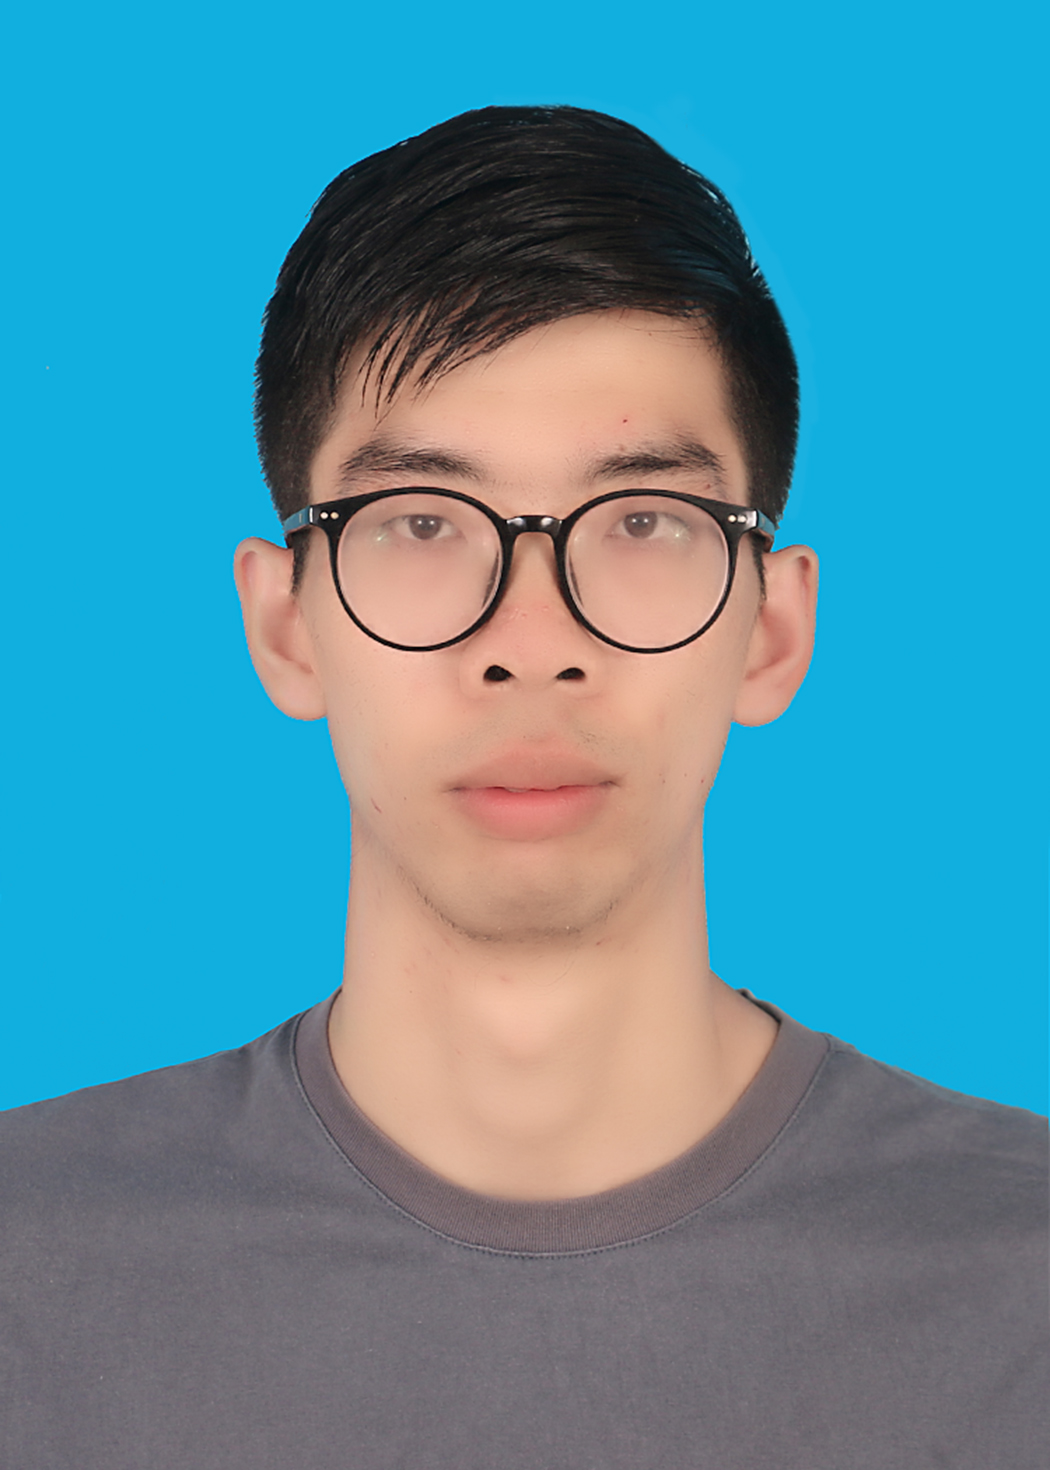
\includegraphics[width=\linewidth]{2}}\end{minipage}}            \\ 
		\cline{1-4}
	   %\begin{tabular}[c]{@{}c@{}}\\ \end{tabular}    
	   出生年月 & 1997.07     & 籍贯     & 江西吉安    &                              \\ 
		\cline{1-4}
		在读学历层次                                               &   硕士研究生%\begin{tabular}[c]{@{}c@{}}\\ \end{tabular}    
		 & 入学日期   & 2021.09 &                              \\ 
		\cline{1-4} {在读专业}                                                  & \multicolumn{3}{c|}{信息与通信工程}   &                              \\ 
		\hline
		身份证号码                                                & \multicolumn{4}{c|}{36243219970725001X}                       \\ 
		\hline
		指导教师姓名                                               & 易见兵         & 研究方向   & \multicolumn{2}{c|}{人体姿态估计}            \\ 
		\hline
		\begin{tabular}[c]{@{}c@{}}本科(硕士)毕\\业学校\end{tabular} & 江西理工大学      & 专业     & \multicolumn{2}{c|}{信息与通信工程}           \\ 
		\hline
		所在院系                                                 & 信息工程学院      & E-mail & \multicolumn{2}{c|}{695449217@qq.com}  \\ 
		\hline
		联系电话                                                 & 18379716287 & 手机     & \multicolumn{2}{c|}{18379716287}       \\ 
		\hline
		\multicolumn{5}{|l|}{二\textbf{\textbf{、项目基本情况}}}                                                                     \\ 
		\hline
		\multicolumn{5}{|l|}{\begin{tabular}[c]{@{}l@{}}项目主要研究内容(2000字以内。文科包括:研究的主要问题目的、意义、研究方法、对\\策建议、创新点等;理工科包括:主要问题、关键技术、解决方案、研究方法、创新点等):\end{tabular}}      \\
		\multicolumn{5}{|l|}{\begin{tabular}[c]{@{}l@{}}\noindent\textbf{2.1 研究背景} \end{tabular}}\\
		
		\multicolumn{5}{|l|}{\begin{tabular}[l]{@{}l@{}} \qquad 人机交互\cite{article}是一门系统与用户之间互动的学科,从上世纪七十年代末,随着人们对它的不\\断认识,逐渐形成了一种多模态形式的人机互动也就是模仿人生活中的交互方式,比如:手\\势、触觉、表情、语音等,让机器也能够获取外界的世界信息,获得视觉感知的能力也就是\\像人类一样能够拥有自己的“眼睛”,所以遇到问题时候是需要机器能够正确理解人类的行为\\,也是在这样的背景下,姿态估计被提出,让它成为了一种当下重要技术之一,而且人体姿态\\估计存在着潜在的应用价值,让学术界、工业界备受关注。\end{tabular}}\\
		
		\multicolumn{5}{|l|}{\begin{tabular}[c]{@{}l@{}}\qquad 姿态估计\cite{DBLP:conf/cvpr/ToshevS14}\cite{DBLP:conf/cvpr/WeiRKS16}\cite{DBLP:conf/eccv/NewellYD16}是计算机视觉中重要任务,也是计算机理解人体的动作、行为不可或缺的一部分。\\姿态估计是过去几十年计算机视觉界一直关注的一个重要问题。姿态估计\cite{DBLP:conf/cvpr/ChenWPZYS18}常常还和姿态识别也\\就是行为识别联系到一起,这是两个概念,行为识别实在最终输出的是图像或者视频的行为的\\类别,而姿态估计是在输入图像视频之后,能都定位到某人的某个身体部位出现的位置,也就\end{tabular}}\\
				
				
				
	
		

		
		\hline
	\end{tabular}
\end{table}
\begin{table}[H]
	\centering
	\renewcommand\arraystretch{1.7}
	\begin{tabular}{|l|}
	\hline
	是能够重建到人体各个部位以及各个关节,估计到人的关节点的坐标,行为识别可以借助姿态\\估计的相关成果来实现。本创新项目主要研究姿态估计,姿态估计大多数是人体姿态估计,还\\有一些有手部姿态估计,手部姿态估计分为有标记和无标记的姿态估计,用于理解手部行为的\\意思。而本创新项目主要围绕人体姿态估计进行阐述。 \\
		
	\begin{tabular} {@{}l@{}}\qquad 目前人体姿态估计已经取得较为不错的效果,它在不断的从二维到三维,从图像到视频,\\从复杂网络到轻量化网络。紧接着又随着深度学习技术的不断发展,将深度学习的许多理论加\\入到了姿态估计。 \end{tabular}\\

	\begin{tabular} {@{}l@{}}\noindent\textbf{2.1.1基于深度学习的姿态估计}\end{tabular}\\

	\begin{tabular}{@{}l@{}}
	\qquad 深度学习时机器学习领域近几年发展较为迅猛的分支。深度学习是自我解释型的学习方式,\\简单方便,功能强大,很多领域都在使用。姿态估计也陆续出现了许多方法,利用深度卷积神\\经网络来增强人体估计系统的性能,在网络架构方面,基于深度学习的姿态估计分为单级网络\\和多级网络,单级网络通常的难点在于后面的特征融合工作,多级网络一般就是重复叠加某个\\细小的小网络结构。单级网络都是会采用特征提取已经训练好的分类网络,微调后作为新网络\\的一个backbone,常用到的网络比如:VGGNet\cite{DBLP:journals/corr/SimonyanZ14a}或ResNet\cite{DBLP:conf/cvpr/HeZRS16}(残差网络)。模型主要有Deeppose\cite{DBLP:conf/cvpr/ToshevS14}\\(直接回归坐标)、CPM\cite{DBLP:conf/cvpr/WeiRKS16}(热力图回归坐标)。对于深度学习的人体姿态估计的算法来讲,大致\\分为自顶向下方法和自底向上的方法。\end{tabular}\\

	\begin{tabular} {@{}l@{}}\noindent\textbf{自顶向下(Top-Down Approaches)}\end{tabular}\\

	\begin{tabular}{@{}l@{}}
	
	
	\qquad 自顶向下这种方法也就是先检测到整个人的存在,再具体检测每个关节点的位置,但是自\\顶向下的缺点有两点,一是对物体检测比较敏感,也就是如果行人未检测出来,关键点就不会\\检测到;
	二是处理量会随着人数的增加而增加,成正比。\\
	
	\qquad 同时它的优点也是很突出:1、召回率较好,因为top-down是先做人体检测,人体往往会比\\部位更大,所以从检测角度来讲会更简单,相应找到的召回率也会更高。2、关键点的定位精度\\会更准,这部分原因是基于裁剪的框,对空间信息有一定的对齐处理,同时因为在做单人估计\\的时候,可以获得一些中间层的上下文信息,对于点的定位是很有帮助的。\\
	\qquad 2017年CVPR采用的自顶向下后,先是使用faster rcnn\cite{DBLP:conf/nips/RenHGS15}当人整体的检测器,其次用一个
	\end{tabular}\\

	\hline
	\end{tabular}

\end{table}
	
\begin{table}[H]
	\centering
	\renewcommand\arraystretch{1.7}
	\begin{tabular}{|l|}
		\hline
	
	\begin{tabular}{@{}l@{}}
	残差网络结构对检测到的人做密集热力图并且预测坐标偏移量,最后将其二者结融合结果得到\\关键点的坐标。同年,MSCOCO比赛的冠军采用级联金字塔网络改进过程,采用多尺度特征\\融合,还用损失函数来处理关键点。肖等人还提供了人体姿态估计的基准方法。自顶向下的检\\测算法有RMPE\cite{DBLP:conf/iccv/FangXTL17},Mask-RCNN\cite{DBLP:conf/iccv/HeGDG17},HRNet\cite{DBLP:conf/cvpr/0009XLW19}。\\
		
	\qquad Regional Multi-Person Pose Estimation(RMPE)\cite{DBLP:conf/iccv/FangXTL17}是上海交大和腾讯优图的论文,被\\ICCV 2017接收。它对于多人姿态估计的方法采用传统的自顶向下的方法,即先检测人,再\\识别人体姿态。检测使用的是SSD-512,识别人体姿态使用的是达到最高水准的Stacked\\ Hourglass\cite{DBLP:conf/eccv/NewellYD16}方法。致力于解决对于不完美的结果,通过调整,使得裁剪的单人能够被单人姿态\\估计方法很好的识别,从而克服检测带来的定位误差。\\
	
	\qquad 对于Mask RCNN\cite{DBLP:conf/iccv/HeGDG17}是一个非常流行的语义和实例分割架构。该模型可以同时预测图像中\\多个物体的候选框位置及分割其语义信息的掩膜。该模型的基础架构很容易被扩展到人体姿态\\估计上来。\\
	
	\qquad 对于HRNet\cite{DBLP:conf/cvpr/0009XLW19}是目前人体姿态估计邻域中最主流的基准网络。为了这些任务位置信息更加\\精准,很容易想到的做法就是维持高分辨率的特征图,事实上HRNet之前几乎所有的网络都\\是这么做的,通过下采样得到强语义信息,然后再上采样恢复高分辨率恢复位置信息,然而这\\种做法,会导致大量的有效信息在不断的上下采样过程中丢失。而HRNet通过并行多个分辨\\率的分支,加上不断进行不同分支之间的信息交互,同时达到强语义信息和精准位置信息的目\\的。\\
		
	\begin{tabular} {@{}l@{}}\noindent\textbf{自底向上(Bottom-Up Approaches)}\end{tabular}\\
	
	
	\qquad 这种方法就是先检测到每个人关节部位的关键点,然后再用图结构、条件随机场等算法组\\接成每个人的姿态,缺点就是将关键点与人关联起来,分组成人具有挑战,而且受遮挡影响太\\大。代表算法:openpose\cite{DBLP:journals/corr/abs-1812-08008},DeepCut\cite{DBLP:conf/cvpr/PishchulinITAAG16},HigherHRNet\cite{DBLP:conf/cvpr/ChengXWSH020}。\\
		
	\qquad OpenPose和很多自底向上的方法一样,OpenPose\cite{DBLP:journals/corr/abs-1812-08008} 首先检测出图像中所有人的关节(关键\\点),然后将检出的关键点分配给每个对应的人。用Part Affinity Fields(PAFs)来学习如何将\\身体关键和个人匹配起来。主要思想是利用贪心算法自下而上的解析步骤从而达到高准确率和实
	\end{tabular}\\

	\hline
	\end{tabular}

\end{table}
	
	
	\begin{table}[H]
		\centering
		\renewcommand\arraystretch{1.7}
		\begin{tabular}{|l|}
		\hline
		\begin{tabular}{@{}l@{}}
	时性。身体部位定位和关联是在两个分支上同时进行的。\\
		
	\qquad 2015 年提出DeepCut\cite{DBLP:conf/cvpr/PishchulinITAAG16}模型,深度卷积预测所有点,再聚类组成图。DeepCut是一个自底向上\\的多人人体姿态估计方法。针对人体姿态估计任务,作者定义了以下问题:1.生成一个由 D 个关节\\候选项组成的候选集合。该集合代表了图像中所有人的所有关节的可能位置。在上述关节候选集中\\选取一个子集。2.为每个被选取的人体关节添加一个标签。标签是 C 个关节类中的一个。每个关节\\类代表一种关节,如“胳膊”“腿”“躯干”等。3.将被标记的关节划分给每个对应的人。\\
	
	\qquad CVPR 2020录用的HigherHRNet\cite{DBLP:conf/cvpr/ChengXWSH020}是一种新的自下而上的人体姿势估计方法,用于使用高分辨率\\特征金字塔学习尺度感知表示。该方法配备了用于训练的多分辨率监督和用于推理的多分辨率聚合,\\能够解决自下而上的多人姿势估计中的尺度变化挑战,并能更精确地定位关键点,尤其是对于小人物。\\HigherHRNet中的特征金字塔包括HRNet的特征图输出和通过转置卷积进行上采样的高分辨率输出。\\
	
	\begin{tabular} {@{}l@{}}\noindent\textbf{2.1.2知识蒸馏}\end{tabular}\\
	\qquad 蒸馏是一种热力学的分离工艺,它利用混合液体或液-固体系中各组分沸点不同,使低沸点组分蒸发\\,再冷凝以分离整个组分的单元操作过程。具体在化学中,蒸馏是一个有效的分离沸点不同的组分的方法\\,大致步骤是先升温使低沸点的组分汽化,然后降温冷凝,达到分离出目标物质的目的。在深度学习中所\\提出的知识蒸馏就是通过引入超参数温度来提高对交叉熵损失中负对数的重视程度。\\
	\qquad \qquad \qquad \qquad \qquad \qquad \qquad \qquad
	\begin{minipage}{0.2\columnwidth}{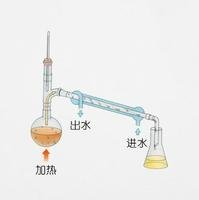
\includegraphics[scale=0.8]{9}}\end{minipage}\\
	\qquad Geoffrey E. Hinton, Oriol Vinyals和Jeffrey Dean\cite{DBLP:journals/corr/HintonVD15}在2015年首次提出了知识蒸馏的概念,学生网\\络从教师提供的基础真实标签和软标签中学习,所以知识蒸馏定义了一种学习方式,在这种学习方式中,\\一个更大的教师网络被用来指导一个更小的学生网络的训练,以完成许多任务。教师网络中蕴涵知识是\\通过教师的软标签传递给学生的。为了提高对负对数的重视,引入了超参数温度。\\
	
	
%	\begin{figure}[H]
%		\centering
%		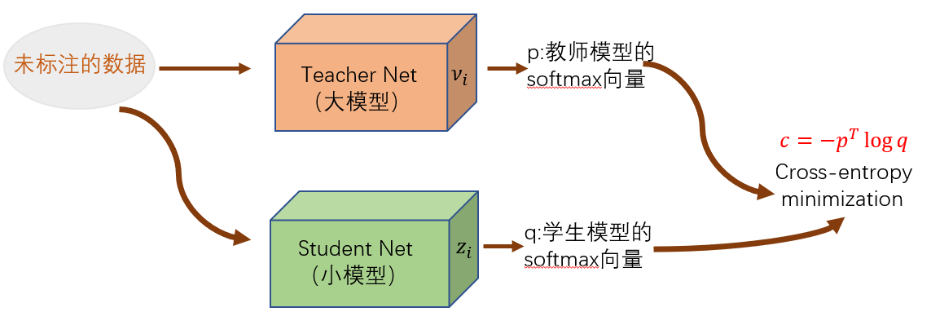
\includegraphics[scale=0.5]{3}
%	\end{figure}
	
	
	\end{tabular}\\

\hline
\end{tabular}

\end{table}

	\begin{table}[H]
	\centering
	\renewcommand\arraystretch{1.7}
	\begin{tabular}{|l|}
		\hline
		\begin{tabular}{@{}l@{}}
\\
	\begin{minipage}{0.2\columnwidth}{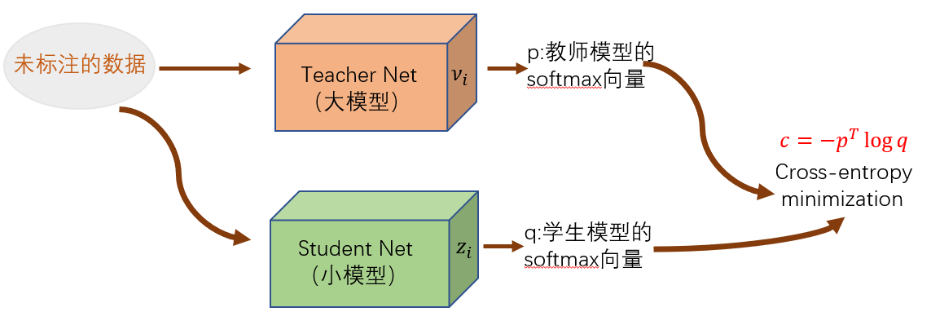
\includegraphics[scale=0.5]{3}}\end{minipage}\\
	\qquad 接下来的工作可以分为两类:logits蒸馏和中间特征\\
	
	\qquad 以往logit精馏的工作主要是提出有效的正则化和优化方法,而不是新颖的方法。DML\cite{DBLP:conf/cvpr/ZhangXHL18}提出了一种\\相互学习的方式,同时培训学生和教师。TAKD\cite{DBLP:journals/corr/abs-1902-03393}引入了一个名为“教师助理”的中型网络,以弥合教师\\和学生之间的差距。\\
	
	\qquad FitNet\cite{DBLP:journals/corr/RomeroBKCGB14}通过一个阶段的中间特征来提取知识。FitNet的想法很简单,通过卷积层将学生的网络特征\\转换为和教师网络模型输出特征的相同形状。用L2距离用来测量它们之间的距离。PKT将教师的知识\\建模为概率分布,用KL散度来测量距离。CRD\cite{DBLP:conf/iclr/TianKI20}将对比学习与知\\识提炼相结合,利用对比目标进行知识转移。\\
	
	\begin{tabular} {@{}l@{}}\noindent\textbf{2.2主要问题}\end{tabular}\\
	
	\qquad 1.最近的研究\cite{DBLP:conf/cvpr/ChengXWSH}已经证明了长期空间依赖性对人体姿态估计的好处。长程空间\\相关性的一般概念是在大视场中对空间信息的全局理解。以前的高分辨率网络\cite{DBLP:conf/cvpr/0009XLW}\cite{DBLP:journals/pami/00010CJDZ0MTW0X21}\cite{DBLP:conf/cvpr/YuXGY0S021}主要依赖于并行分支中深度叠加的卷积层提取多尺度特征\\来构建空间相关性,但受宽度和深度的限制,轻量级网络的容量会受到严重影响。因此,其中一个问题\\是如何增强轻量级高分辨率网络,以更有效的方法建模长程空间依赖性。\\
	
	\qquad 2.我们观察到,最先进的人体姿态估计基础网络(如HRNet\cite{DBLP:conf/cvpr/0009XLW19})的基本CNN构建模块在建立大型网\\络时并不具有成本效益,因为每层有大量的通道,而且更难训练。并且在后续的边缘设备进行部署时有\\对于边缘设备较高的要求,不利于批量部署操作。在本研究中,我们考虑在不降低模型性能的情况下提\\高人体姿态估计效率,但保留可比较的精度结果的问题。\\
	
		\end{tabular}\\

\hline
\end{tabular}
	

	
	
	
\end{table}
		\begin{table}[H]
		\centering
		\renewcommand\arraystretch{1.7}
		\begin{tabular}{|l|}
			\hline
			\begin{tabular}{@{}l@{}}
				

	\qquad 3.目前还不清楚PSAM\cite{DBLP:journals/corr/abs-2107-00782}如何使嵌入分类和置换的像素级回归得到最大的好处。在复杂的DCNN头部\\回归,如那些在,无锚的人体姿态检测任务。据我们所知,大多数现有的工作与自我注意块只插入块骨干\\网络。我们未来的工作是探索PSAM在DCNN头部的应用。\\
	\begin{tabular} {@{}l@{}}\noindent\textbf{2.3 关键技术}\end{tabular}\\
			
	\begin{tabular} {@{}l@{}}\noindent\textbf{2.3.1极化自注意力模块(PSAM)}\end{tabular}\\	
	\qquad 注意力机制(Attention Mechanism)是人们在深度学习模型中嵌入的一种特殊结构,用来自动学习和\\计算输入数据对输出数据的贡献大小。注意力机制是上世纪九十年代,一些科学家在研究人类视觉时,发\\现的一种信号处理机制。人工智能领域的从业者把这种机制引入到一些模型里,并取得了成功。目前,注\\意力机制已经成为深度学习领域,尤其是自然语言处理领域,应用最广泛的“组件”之一。这两年曝光度\\极高的BERT\cite{DBLP:journals/corr/abs-2007-01127}、GPT\cite{Radford2018ImprovingLU}、Transformer\cite{DBLP:journals/corr/abs-1810-04805}等等模型或结构,都采用了注意力机制。\\
	
	\qquad 一些学者尝试让模型自己学习如何分配自己的注意力,即为输入信号加权。他们用注意力机制的直接\\目的,就是为输入的各个维度打分,然后按照得分对特征加权,以突出重要特征对下游模型或模块的影响\\。这也是注意力机制的基本思想。\\
	
	\qquad 自注意块作用于输入张量X来突出或抑制特征,这很像光学透镜过滤光线。在摄影中,横向方向上\\总是有随机的光线产生眩光/反射。偏振滤波,只允许光通过正交于横向方向,可以潜在地提高照片的对\\比度,由于总强度的损失,滤波后的光通常有一个小的动态范围,因此需要额外的增强。我们借用摄影的\\关键因素,提出了极化自我注意(PSA)机制:\\
	
	\qquad (1)滤波:在一个方向上完全折叠特征,同时保持其正交方向上的高分辨率;\\
	\qquad (2)高动态范围:在瓶颈张量(注意块中最小的特征张量)处进行Softmax归一化,增加注意的动态范\\围,然后进行色调映射Sigmoid函数。形式上,我们将PSA机制\cite{DBLP:journals/corr/abs-2107-00782}实例化为下面的PSA块:\\
	
	\begin{tabular} {@{}l@{}}\noindent\textbf{仅通道注意力分支:}\end{tabular} \quad $A^{ch}(X) \in \mathcal{R}^{C\times 1\times 1}$\\
	
	\qquad \qquad \qquad \qquad \qquad \qquad  $A^{ch}(X)=F_{SG}[W_{z|\theta_1}(\sigma_1(W_v(X))\times F_{SM}(\sigma_2(W_q(X))))]$\\
	
	$W_z,W_q,W_v$是三个(1 x 1)卷积核,它们学习不同通道之间空间特征的线性组合。$\sigma_1$ 和$\sigma_2$ 两个张量变形\\算符。$F_{SM}$是SoftMax操作而$\times$是矩阵点积运算。\\
	
	
	
	
	
	\end{tabular}\\

	\hline
	\end{tabular}

\end{table}
	\begin{table}[H]
	\centering
	\renewcommand\arraystretch{1.7}
	\begin{tabular}{|l|}
		\hline
		\begin{tabular}{@{}l@{}}
	\qquad 仅通道分支的输出为$Z^{ch}=A^{ch}(X)\odot^{ch}X\in \mathcal{R}^{C\times H\times W}$,$\odot^{ch}$是一个基于通道的乘法运算符。\\
	\qquad \qquad \qquad \qquad \qquad \qquad \qquad \qquad \begin{minipage}[c]{0.2\columnwidth}{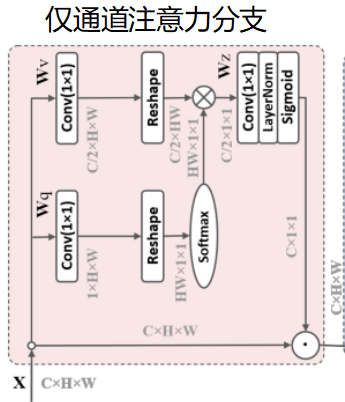
\includegraphics[scale=0.5]{4}}\end{minipage}\\
	
	\begin{tabular} {@{}l@{}}\noindent\textbf{仅空间注意力分支:}\end{tabular} \quad  $A^{sp}(X) \in \mathcal{R}^{1\times H\times W}$\\
	
	\qquad \qquad \qquad \qquad \qquad \qquad 
	$A^{sp}(X)=F_{SG}[\sigma_3(F_{SM}(\sigma_1(F_{GP}(W_q(X))))\times \sigma_2(W_v(X)))]$\\
	
	$W_q$和$W_v$是分别标准的$1\times 1$卷积层。$\sigma_1$,$\sigma_2$和$\sigma_3$是三个张量变形算符。$F_{SM}$是SoftMax操作, $F_{GP}$是\\一个全局池操作符。$\times$是矩阵点积运算。\\
	
	\qquad 仅空间分支的输出为$Z^{sp}=A^{sp}(X)\odot^{sp}X\in \mathcal{R}^{C\times H\times W}$,$\odot^{sp}$是一个空间相关的乘法运算符。\\
	
	\qquad \qquad \qquad \qquad \qquad \qquad \qquad \qquad \begin{minipage}[c]{0.2\columnwidth}{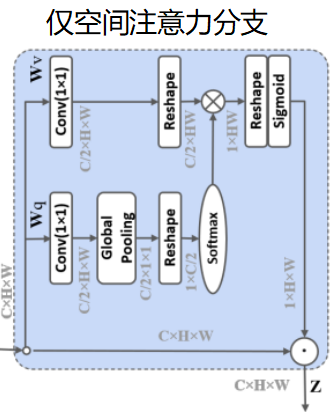
\includegraphics[scale=0.5]{5}}\end{minipage}\\

	\begin{tabular} {@{}l@{}}\noindent\textbf{整体注意力模块:}\end{tabular}\\
	\qquad \qquad \qquad \qquad \qquad \qquad$PSAM(X) = Z^{sp}(Z^{ch}) = A^{sp}(A^{ch}(X)\odot^{ch}X)\odot^{sp}A^{ch}(X)\odot^{ch}X$
	\\
	

\end{tabular}\\

\hline
\end{tabular}

\end{table}
		\begin{table}[H]
		\centering
		\renewcommand\arraystretch{1.7}
		\begin{tabular}{|l|}
			\hline
			\begin{tabular}{@{}l@{}}
				\\
	\qquad \qquad \qquad \qquad \begin{minipage}[c]{0.2\columnwidth}{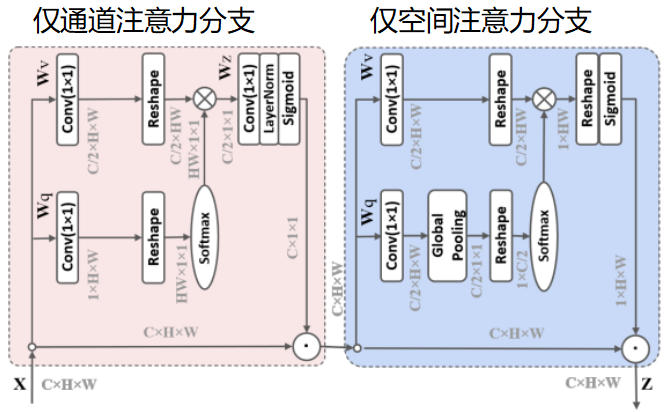
\includegraphics[scale=0.5]{7}}\end{minipage}\\
	\qquad 具体点我们在每个Residual块的第一个$3\times3$卷积后添加PSAM。但是目前还不清楚PSAM如何才\\能从嵌入分类的像素级回归中获益在复杂的DCNN头部。据我们所知,大多数现有的工作与自我注意块只\\插入块骨干网络。我们工作是还会探索PSAM在DCNN头部位置中的应用。\\
				
	\qquad PSAM与其他自我注意模块的关系: 我们将PSAM加入到表1中进行对比,PSA模块相对现有的注\\意力模块更先进的原因:\\
	
	\qquad (1) 内部分辨率 vs 复杂性: 与最高配置下的现有注意力块相比,PSA 在两个分支上都保持了最高的\\注意力分辨率 $(C/2)^3$ 和空间 $([W, H])$维度。此外,在我们只关注通道的情况下,将 Softmax重加权与\\挤压激励融合,利用 Softmax 作为瓶颈张量$C/2 \times W \times h$的非线性激活。通道数$C − C/2 − C$遵循挤压\\激励模式,这对GC块和SE块都有利。我们的设计实现了高分辨率的压缩激励,同时计算复杂度可与\\GC块相当。\\
	
	\qquad (2) 我们只关注空间的注意力不仅保持了饱满$[W, H]$ 空间分辨率,而且内部保持$2\times 𝐶\times 𝐶/2$ 在$W_q$\\和 $W_v$ 中可学习的参数,用于非线性 Softmax 重加权,这是比现有块更强大的结构。\\
	
	\qquad (3) 输出为非线性分布。PSAM仅通道和仅空间分支都使用 Softmax 和 Sigmoid 组合。将 Softmax\\和 Sigmoid 进行组合作为概率分布函数,考虑关键点热图可以在线性变换上近似。因此,我们期望非线\\性可以充分利用保存在内部的高分辨率信息PSAM注意分支。\\
	NL\cite{DBLP:conf/cvpr/0004GGH},GC\cite{DBLP:conf/iccvw/0001XLWH},SE\cite{DBLP:conf/nips/HuSASV18},CBAM\cite{DBLP:conf/eccv/WooPLK},DA\cite{DBLP:conf/cvpr/FuLT0BFL},EA\cite{DBLP:conf/wacv/ShenZZY}\\
	
	
	
	
	
	\end{tabular}\\

	\hline
	\end{tabular}

		\end{table}


		\begin{table}[H]
	\centering
	\renewcommand\arraystretch{1.7}
	\begin{tabular}{|l|}
		\hline
		\begin{tabular}{@{}l@{}}
			\\
		\qquad \qquad \qquad\begin{minipage}[c]{0.2\columnwidth}{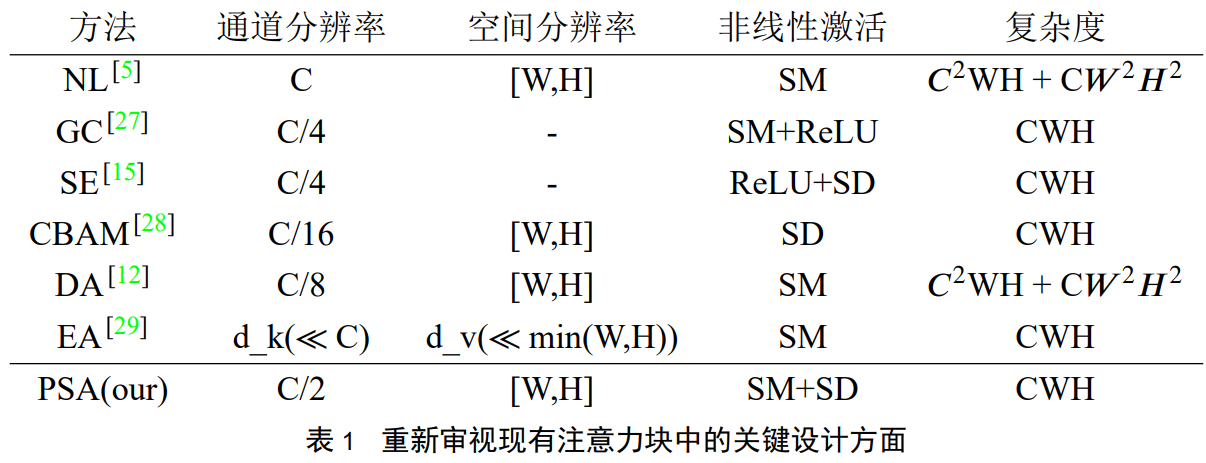
\includegraphics[scale=0.3]{6}}\end{minipage}\\
			
	\begin{tabular} {@{}l@{}}\noindent\textbf{2.3.2知识蒸馏(Distilling Knowledge)}\end{tabular}\\
		\qquad 训练过程相当于一个有几十年经验的老师(水平高,知识全面,学的快等特点)相当于大模型,有\\个刚入学的学生(知识储备能力小,经验不丰富)相当于小模型。让教师网络指导学生网络进行训练。\\
	\qquad \qquad \qquad \qquad \qquad 
	\begin{minipage}[c]{0.2\columnwidth}{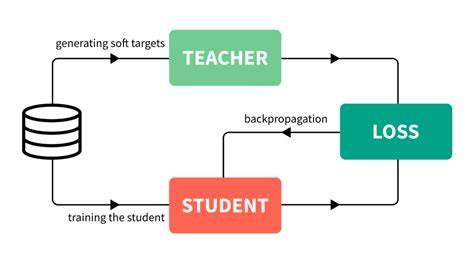
\includegraphics[scale=0.6]{10}}\end{minipage}\\
	\qquad \qquad \qquad \qquad \qquad \qquad \qquad \qquad \qquad \qquad 知识蒸馏整体过程\\
			
	\qquad 一旦训练了繁琐的模型,我们就可以使用另一种训练方式,我们称之为“蒸馏”,将知识从繁琐的\\模型转移到更适合部署的小模型。一般认为,用于训练的目标函数应尽可能接近地反映使用者的真实目\\标。对于这个转移阶段称为知识蒸馏过程,我们可以使用相同的训练集,也可以使用单独的数据集。当\\繁琐的模型是简单模型的大集合时,我们可以使用它们各自预测分布的算术或几何平均值作为软目标。\\当软目标有很高的熵,他们提供更多的信息/培训情况比硬目标和更少的方差之间的梯度训练情况,所以小\\模型通常可以比原来繁琐的模型训练更少的数据和使用更高的学习速率\cite{DBLP:conf/kdd/BucilaCN06}。\\

\qquad 繁琐的模型几乎总是以很高的置信度产生正确的答案,学习函数的很多信息都存在于软目标中非常小\\的概率的比率中。在最简单的精馏形式中,知识通过在一个转移集上对其进行训练,并对通过在其soft-\\max中使用高温的繁琐模型产生的转移集中的每个情况使用软目标分布来转移到精馏模型。训练蒸馏模
\end{tabular}\\

\hline
\end{tabular}

\end{table}


\begin{table}[H]
	\centering
	\renewcommand\arraystretch{1.7}
	\begin{tabular}{|l|}
		\hline
		\begin{tabular}{@{}l@{}}
	\hline
	\qquad \qquad \qquad  
	\begin{minipage}[c]{0.2\columnwidth}{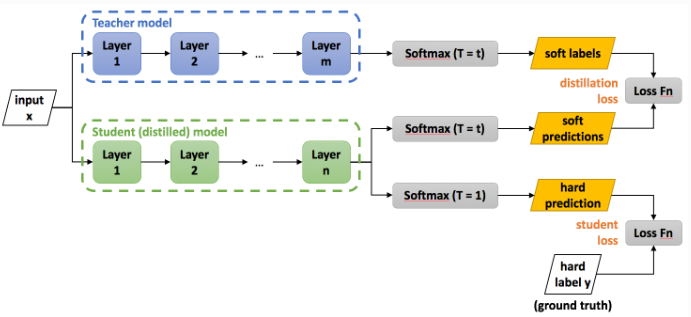
\includegraphics[scale=0.5]{11}}\end{minipage}\\
	
	\qquad \qquad \qquad \qquad \qquad \qquad \qquad \qquad \qquad 目标检测知识蒸馏整体过程\\
	型时使用相同的高温,但训练后使用的温度为1。\\
	\qquad 在目标识别领域中。原来我们需要让新模型的softmax分布与真实标签匹配,现在只需要让新模型与\\原模型在给定输入下的softmax分布匹配了。直观来看,使用知识蒸馏比前者具有这样一个优势:经过训\\练后的原模型,其softmax分布包含有一定的知识——真实标签只能告诉我们,某个图像样本是一辆宝马\\,不是一辆垃圾车,也不是一颗萝卜;而经过训练的softmax可能会告诉我们,它最可能是一辆宝马,不\\大可能是一辆垃圾车,但绝不可能是一颗萝卜。而这些信息对于学生网络模型的学习是具有正向的促进作\\用。\\
	
	\qquad 接续前面的讨论,我们的目标是让新模型与原模型的softmax输出的分布充分接近。直接这样做是有\\问题的:在一般的softmax函数中,自然指数$e$先拉大logits之间的差距,然后作归一化,最终得到的分\\布是一个arg max的近似 ,其输出是一个接近one-hot的向量,其中一个值很大,其他的都很小。这种情\\况下,前面说到的"可能是垃圾车,但绝不是萝卜"这种知识的体现是非常有限的。相较类似one-hot这\\样的硬性输出,我们更希望输出更"软"一些。\\
	
	\qquad 一种方法是直接比较logits来避免这个问题。具体地,对于每一条数据,记原模型产生的某个logits\\$v_i$是 ,新模型产生的logits是$z_i$,我们需要最小化\\
	\qquad \qquad \qquad \qquad \qquad \qquad \qquad \qquad \qquad \qquad
	\LARGE{$D = \frac{1}{2}(z_i - v_i)^2$}\\
	\qquad 文献\cite{DBLP:journals/corr/HintonVD15}中提出了更通用的一种做法。考虑一个广义的softmax函数:\\
	\qquad \qquad \qquad \qquad \qquad \qquad \qquad \qquad \qquad \qquad
	\LARGE{$q_i = \frac{exp(z_i/T)}{\sum_{j}exp(z_j/T)}$}\\
	其中$T$是温度,这是从统计力学中的玻尔兹曼分布中借用的概念。容易证明,当温度$T$趋向于0时,soft-\\
		\end{tabular}\\
	
\hline
\end{tabular}

\end{table}

\begin{table}[H]
	\centering
	\renewcommand\arraystretch{1.7}
	\begin{tabular}{|l|}
		\hline
		\begin{tabular}{@{}l@{}}
		\hline	
	max输出将收敛为一个one-hot向量,温度$T$趋向于无穷时,softmax的输出则更“软”。具体地,在训练\\时我们需要最小化两个分布的交叉熵(Cross-entropy),记新模型利用softmax函数公式所产生的分布是$q$,\\而原模型产生的分布是$p$,则我们需要最小化:\\
	\qquad \qquad \qquad \qquad \qquad \qquad \qquad \qquad \qquad \qquad
	\LARGE{$C = -p^Tlogq$}\\
	\qquad 转移集中的每一种情况都贡献了教师模型和学生模型输出的交叉熵梯度其对某一个logit $z_i$的梯度:\\($z_i$相对于蒸馏模型的每个logit, $v_i$教师模型的logits, $p_i$产生软目标概率, $T$是在有温度调节的情况下进行\\转移训练):\\
	 \qquad \qquad \qquad \qquad \qquad
	\huge{$\frac{\partial C}{\partial z_i} = \frac{1}{T}(q_i-p_i) = \frac{1}{T}(\frac{e^{z_i/T}}{\sum_{j}e^{z_i/T}}-\frac{e^{v_i/T}}{\sum_{j}e^{v_i/T}})$}\\
	
	如果温度高于对数的量级:\\
	\qquad \qquad \qquad \qquad \qquad \qquad \qquad
	\huge{$\frac{\partial C }{\partial z_i} = \frac{1}{T}(\frac{1 + z_i/T}{N + \sum_{j}z_i/T}-\frac{1 + v_i/T}{N + \sum_{j}v_i/T})$}	\\
	
	如果我们现在假设所有logits对每个样本都是零均值化的(即 $\sum_{j}z_j = \sum_{j}v_j = 0$),那么:\\
	\qquad \qquad \qquad \qquad \qquad \qquad \qquad \qquad \qquad
	\huge{$\frac{\partial C }{\partial z_i} = \frac{1}{NT^2}(z_i-v_i)$}\\
	在较低的温度下,蒸馏很少注意匹配比平均值相差得多的对数。另一方面,但是比平均值相差得多的对数\\可能会传递由繁琐的模型获得的知识的有用信息。\\
	
	\qquad 知识蒸馏和最小化logits的平方差是等价的(因为梯度大致是同一个形式)。实验表明,温度不能取太\\大,而应该使用某个适中的值,这表明忽略极负的logits对新模型的表现很有帮助(较低的温度产生的分布\\比较“硬”,倾向于忽略logits中极小的负值)。\\
	\begin{tabular} {@{}l@{}}\noindent\textbf{通过知识蒸馏加强监督}\end{tabular}\\
		
	\qquad 我们采用知识精馏的通用模型训练策略:\\
	\qquad1.我们先训练一个老师模型。在我们的实验中,默认我们选择了原始的HigherHRNet模型[16],因\\为它设计干净,模型鲁棒性强,可以不受任何限制地考虑其他更强的模型。它是目前人体姿态估计中精度\\最高的模型。\\
	\qquad2. 然后,我们利用教师模型学习到的知识来训练目标学生模型。知识的提炼发生在这一步。\\


	\end{tabular}\\
\hline
\end{tabular}

\end{table}

\begin{table}[H]
	\centering
	\renewcommand\arraystretch{1.7}
	\begin{tabular}{|l|}
		\hline
		\begin{tabular}{@{}l@{}}
	\qquad 我们为了描述整个学生网络训练过程的概貌,将知识蒸馏主要步骤呈现如图1所示,并之后进行分阶\\段介绍。\\
	\begin{minipage}[c]{0.2\columnwidth}{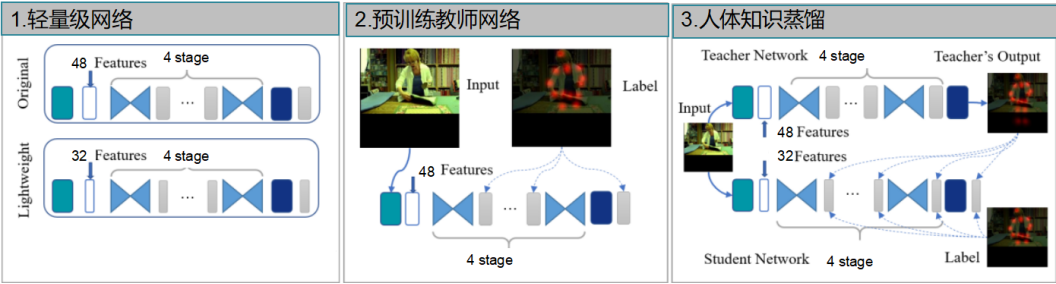
\includegraphics[scale=0.45]{12}}\end{minipage}\\
	\qquad \qquad  \qquad \qquad \qquad \qquad  \qquad \qquad \qquad \qquad  知识蒸馏主要步骤 \\
	
	\textbf{阶段一:}设置轻量级网络。\\
	\begin{minipage}[c]{0.6\columnwidth}{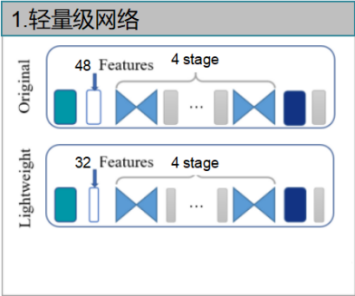
\includegraphics[scale=0.45]{13}}\end{minipage}\begin{minipage}[c]{0.4\columnwidth}
		\qquad 原始的网络结构通过Stem后变为通道数为48的特征图,之后下采样后通道数翻倍,长宽减半。而轻量级的网络结构通过后变为通道数为32的特征图,之后下采样后通道数翻倍,长宽减半。而两者的stage数都为4。
	\end{minipage}\\
	\textbf{阶段二:}预训练教师网络。\\
	\begin{minipage}[c]{0.6\columnwidth}{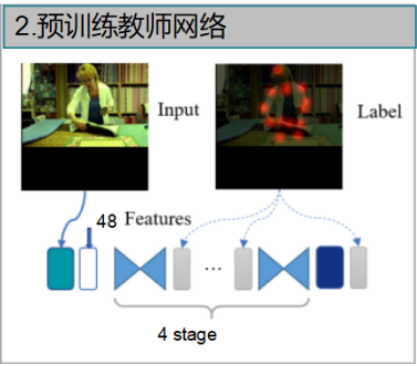
\includegraphics[scale=0.45]{14}}\end{minipage}\begin{minipage}[c]{0.4\columnwidth}
		\qquad 教师网络结构通过Stem后变为通道数为48的特征图,之后下采样后通道数翻倍,长宽减半。\\

		\qquad 训练过程是通过网络预测的关键点位置和真实关键点位置信息做$L_2$范数,并将其作为损失函数。在训练过程中实时对其进行反向传播,进而优化权重参数。

	\end{minipage}\\
	\textbf{阶段三:}人体知识蒸馏。\\
	
		\end{tabular}\\
\hline
\end{tabular}

\end{table}

\begin{table}[H]
	\centering
	\renewcommand\arraystretch{1.7}
	\begin{tabular}{|l|}
		\hline
		\begin{tabular}{@{}l@{}}
	\begin{minipage}[c]{0.6\columnwidth}{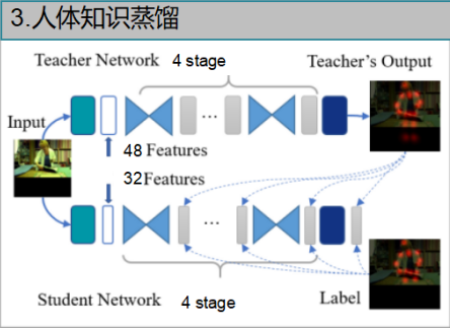
\includegraphics[scale=0.45]{15}}\end{minipage}\begin{minipage}[c]{0.5\columnwidth}
		\qquad 将输入的图片分别放入教师模型和学生模型中进行训练,教师的网络结构通过Stem后变为通道数为48的特征图,之后下采样后通道数翻倍,长宽减半。而学生的网络结构通过后变为通道数为32的特征图,之后下采样后通道数翻倍,长宽减半。

	\end{minipage}\\
	\qquad 为了提炼老师原有的知识来对学生模型进行训练的关键点是设计一个适当的蒸馏损失函数,使得能\\够有效地提取和转移教师的知识到学生模型的训练过程中。我们将通过教师网络预测的关键点位置和真\\实关键点位置信息做L2范数和教师网络预测的关键点位置和学生网络预测的关键点位置做L2范数,\\并将两个损失函数作为损失函数。\\
	\qquad 对于传统的人体姿态模型训练过程中,我们通常使用基于损失函数的均方误差(Mean-Squared Error,\\MSE)[27][28]。为了表示真实人体关节标签,我们为每个关节k生成一个置信图$m_k(k\in{1,···,k})$,通过\\将高斯核核以标记位置$z_k = (x_k, y_k)$为中心。更具体地说,第k个关节标号的高斯置信映射$m_K$可以写\\成:\\
	\qquad \qquad \qquad
	\huge{$m_k(x,y) = \frac{1}{2\pi \sigma^2}exp(\frac{-[(x-x_k)^2 + (y-y_k)]^2}{2\sigma^2})$}\\
	其中$(x, y)$表示像素位置,超参数$\sigma$表示预先确定的空间方差。则得到MSE损失函数为:\\
	\qquad \qquad \qquad \qquad \qquad \qquad
	\huge{$\mathcal{L}_{mse} = \frac{1}{K}\sum_{k=1}^{K}\left \| m_k - \hat{m}_k \right \|^2_2$}\\
	其中$m_k$表示第k个关节的预测置信图,$\hat{m}_k$表示第k个关节的真实位置。\\
	
	\qquad 在此之前的蒸馏函数设计都是用于对象分类环境下的单标签softmax交叉熵损失[3,13]中,不适合在\\2D图像空间中传递结构化的人体姿态知识。为了解决上述问题,我们设计了一个联合置信度图专用姿态蒸\\馏损失函数,公式为:\\
	\qquad \qquad \qquad \qquad \qquad \qquad
	\huge{$L_{kd} = \frac{1}{K} \sum_{k=1}^{K}\left \| m^s_k - m^t_k\right \|^2_2$}\\
	式中,$m^s_k$和$m^t_k$分别为预先训练的教师模型和受训的学生目标模型预测的对第K个关节信息的置信图。\\我们选择MSE函数作为蒸馏的损失函数,用来衡量学生和教师模型之间的分歧,以最大化与姿势监督学\\习损失的可比性。\\
	
	\end{tabular}\\
	\hline
	\end{tabular}

\end{table}
\begin{table}[H]
	\centering
	\renewcommand\arraystretch{1.7}
	\begin{tabular}{|l|}
		\hline
		\begin{tabular}{@{}l@{}}
	\qquad 对于学生模型的损失函数还是使用传统的MSE函数作为损失函数。\\
	\qquad 我们将训练过程中人体姿态估计使用知识精馏的整体损失函数表示为:\\
	\qquad \qquad \qquad \qquad \qquad \qquad
	\huge{$\mathcal{L}_{total} = \alpha\mathcal{L}_{kd} + (1-\alpha)\mathcal{L}_{mse}$}\\
	其中$\alpha$为两个损失项之间的平衡权重,通过交叉验证估计。\\
	\begin{tabular} {@{}l@{}}\noindent\textbf{2.4 解决方案}\end{tabular}\\
	\qquad 该项目用Python语言进行编程,将项目的数据集调用进项目网络结构中进行各个深度卷积神经网络\\权重学习操作。\\
	\qquad (1)针对如何更有效的使用人体姿态知识蒸馏这一训练策略,可通过现阶段关于目标识别中的做法类比\\于人体姿态估计这一具体的任务中。更重要的是理解人体姿态估计这一领域中已经采用的蒸馏方法,具体\\这一训练策略的可行性要通过实验数据和理论方面进行验证确定。对人体姿态知识蒸馏中的损失函数设置\\做相关的消融实验。\\
	\qquad (2)在现阶段轻量级模型的基础上,对于轻量级模型,添加先阶段泛化能力很好的注意力模块,提高轻\\量级网络整体的准确性。对于要加入的注意力模块,将有意的进行讨论PSAM如何才能从嵌入分类的像素\\级回归中获益在复杂的DCNN头部。据我们所知,大多数现有的工作与自我注意块只插入块骨干网络。我\\们工作是还会探索PSAM在DCNN头部位置中的应用。\\
	\qquad (3)对于整体的网络结构尾部,加入现阶段泛化能力很好的反卷积模块,用于生成比输入特征图分辨率\\高的高质量特征图,重新组合各个阶段生成的特征图,从各个特征图中学习到不同维度的信息,进而提高\\轻量级网络整体的准确性。\\
	
	\begin{tabular} {@{}l@{}}\noindent\textbf{2.5 研究方法}\end{tabular}\\
	\qquad 首先我们建立适合程序运行的实验平台和环境,Ubuntu系统,Pytorch深度学习框架等。在这个平台\\和环境上进行方法和技术的研究,对课题研究内容进行整体框架规划分析和设计,合理安排各阶段任务和\\分配有限资源,部分设计各个击破。该项目的研究方法及过程如下图所示。\\
	
		\end{tabular}\\
			\hline
		\end{tabular}
		
\end{table}

\begin{table}[H]
	\centering
	\renewcommand\arraystretch{1.7}
	\begin{tabular}{|l|}
		\hline
		\begin{tabular}{@{}l@{}}
			\qquad \qquad \qquad  \qquad \qquad \qquad  \qquad \qquad \qquad  \qquad \qquad \qquad  \qquad \qquad \qquad  \qquad \qquad \qquad  \qquad \qquad \qquad  \qquad \qquad \qquad  \\

			\qquad \qquad  \qquad  
			\begin{minipage}[c]{0.2\columnwidth}{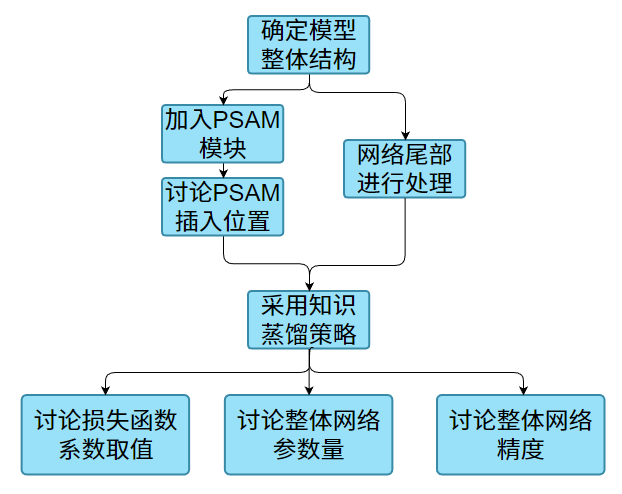
\includegraphics[scale=0.56]{16}}\end{minipage}\\
			\qquad \qquad  \qquad \qquad \qquad  \qquad \qquad \qquad  \qquad \qquad 项目的整体研究过程
		\end{tabular}\\
	\qquad 1、确定模型整体结构。\\
	\qquad 我们采用在IJCAI上发表的最新动态轻量级的高分辨率网络(Dite-HRNet\cite{DBLP:journals/corr/abs-2204-10762}),可以高效地提取多尺度\\上下文信息和建立人体姿态估计的长期空间依赖性模型。实验结果表明,该网络在COCO和MPII人体\\姿态估计数据集上都取得了优异的性能,超过了目前最先进的轻量级网络。Dite-HRNet的整体网络结构\\如下图所示。\\
	  
	\begin{minipage}[c]{0.2\columnwidth}{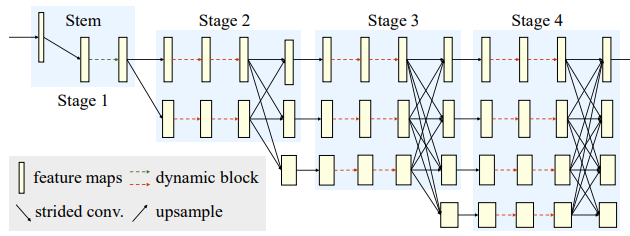
\includegraphics[scale=0.75]{17}}\end{minipage}\\
	\qquad \qquad  \qquad \qquad \qquad  \qquad \qquad \qquad  \qquad \qquad Dite-HRNet整体网络结构\\
	
	
	
	
	\hline
\end{tabular}

\end{table}
\begin{table}[H]
	\centering
	\renewcommand\arraystretch{1.7}
	\begin{tabular}{|l|}
		\hline
		\begin{tabular}{@{}l@{}}
			\qquad 2.加入PSAM模块。  \\
			\qquad 为了提高网络结构对于特征图信息的学习能力,而注意机制在深卷积神经网络(DCNN)已经成为流行\\推动特征图信息中远程依赖关系,特定于像素级别的关注。而PSAM模块似乎已经耗尽了其仅限通道和仅\\限空间分支的表示能力。实验结果表明,在二维人体姿态估计基准上,加入PSAM模块有所提高。模型的\\整体网络结构如下图所示。 目前还不清楚PSAM如何才能使嵌入在复杂的DCNN头部像素级回归得到最\\大的好处。据我们所知,大多数现有的自注意块工作只在骨干网中插入自注意块。我们将讨论PSAM插入\\进DCNN其他位置的使用。\\
			
			\begin{minipage}[c]{0.2\columnwidth}{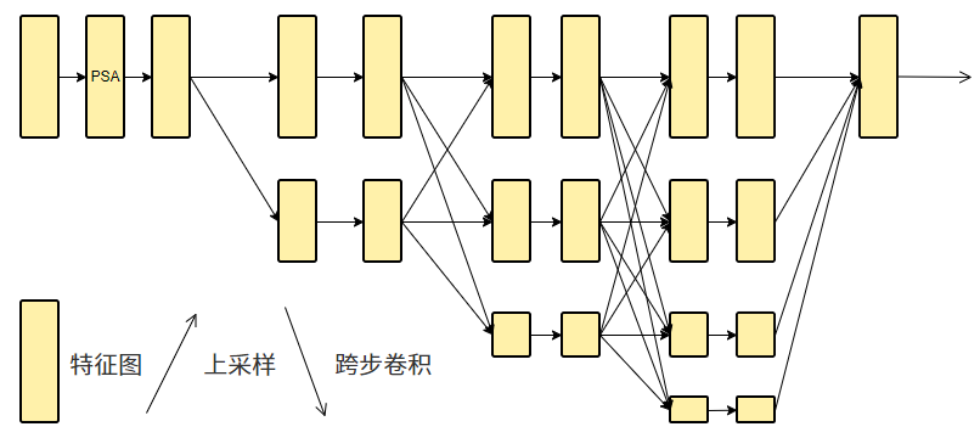
\includegraphics[scale=0.55]{18}}\end{minipage}\\
			\qquad \qquad  \qquad \qquad \qquad  \qquad \qquad \qquad  \qquad \qquad 模型整体网络结构\\
			\qquad 3.模型网络尾部进行处理。\\
			\qquad 在整体网络结构的尾部采用PP-PicoDet\cite{DBLP:journals/corr/abs}提出了CSP-PAN结构,使用1*1的卷积将特征的通道数\\与BackBone输出的最小通道数进行统一,从而减少计算量,并保证特征融合性能不受影响。此外,PP\\-PicoDet还在CSP-PAN的基础上再下采样一次,添加一个更小的特征尺度来提升大物体的检测效果。\\
			
			\qquad 与此同时,PP-PicoDet在Neck和Head部分均采用深度可分离卷积,将$3x3$卷积核增大至$5×5$,\\来增大感受野,还保持了速度不变。并且PP-PicoDet采用了通道数和Neck一致的“耦合头”,相比于\\小通道数的“解耦头”有更快的预测速度。\\
			
					\end{tabular}\\
		\hline
	\end{tabular}

\end{table}
\begin{table}[H]
		\centering
		\renewcommand\arraystretch{1.7}
		\begin{tabular}{|l|}
			\hline
			\begin{tabular}{@{}l@{}}	
			
			\qquad 我们使用PAN[41]结构得到多级特征映射,使用CSP结构对相邻特征映射进行特征拼接和融合。整\\体网络的尾部使用CSP-PAN模块进行特征的融合,在原有的CSP-PAN中,每个输出特征图中的通道号\\与骨干输入的通道号保持一致。对于移动设备来说,信道数大的结构具有昂贵的计算成本。我们通过使所\\有特征图中的所有信道数等于$1\times1$卷积的最小信道数来解决这个问题。整体修改后的CSP网络结构插入\\整体网络结构的尾部。\\
			\qquad \qquad  \qquad 
			\begin{minipage}[c]{0.2\columnwidth}{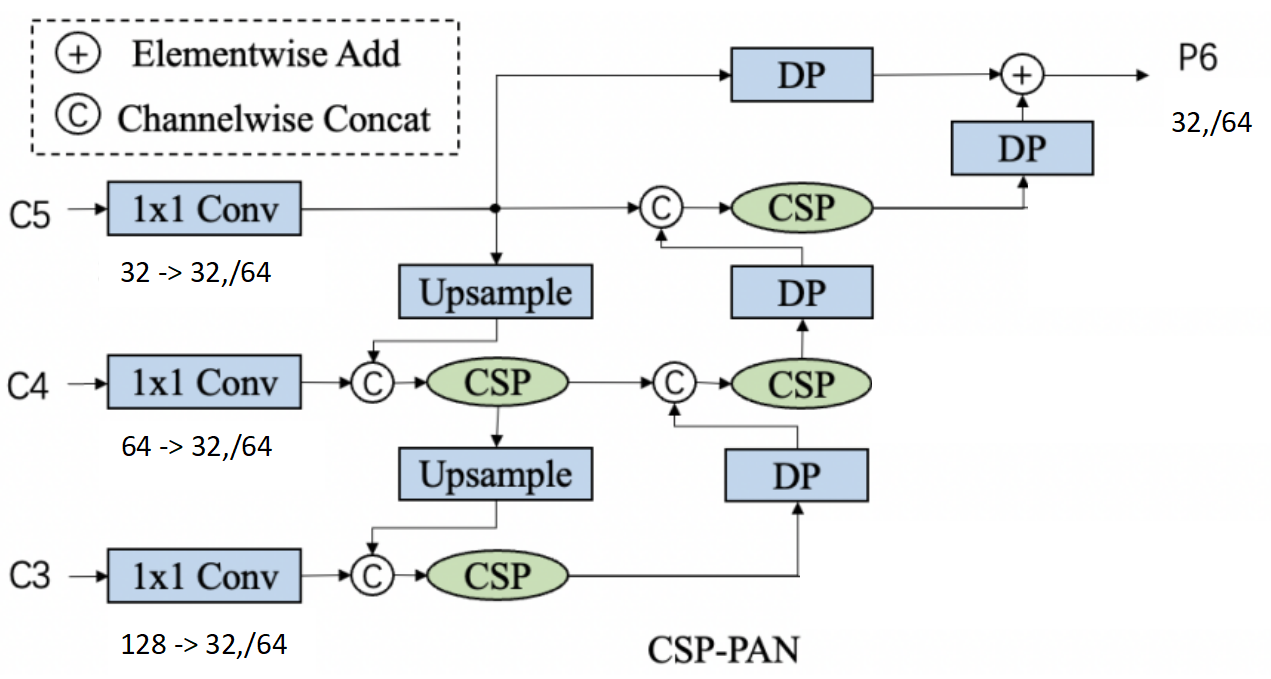
\includegraphics[scale=0.32]{20}}\end{minipage}\\
			\qquad \qquad  \qquad \qquad \qquad  \qquad \qquad \qquad 轻量级的CSP-PAN模块插入网络尾部\\
			\qquad \qquad  \qquad \qquad \qquad  \qquad \qquad \qquad  
			\begin{minipage}[c]{0.2\columnwidth}{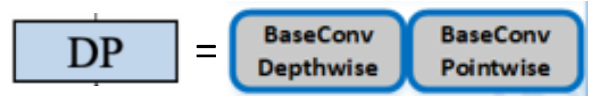
\includegraphics[scale=0.32]{21}}\end{minipage}\\
			\qquad \qquad  \qquad \qquad \qquad  \qquad \qquad \qquad  \qquad DP模块采用了深度卷积和点卷积\\
			\qquad 该轻量级的CSP模块的整体结构如下图所示。\\
			\qquad \qquad  \qquad \qquad  
			\begin{minipage}[c]{0.2\columnwidth}{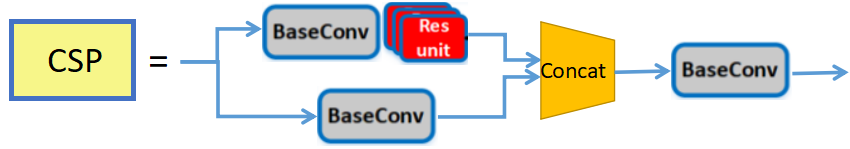
\includegraphics[scale=0.4]{22}}\end{minipage}\\
			\qquad \qquad  \qquad \qquad \qquad  \qquad \qquad \qquad  \qquad CSP模块采用了深度卷积和点卷积\\
			\qquad 我们修改了现阶段泛化性较好的轻量级物体探测器,在移动设备的物体检测方面具有卓越的性能。将\\该网络模块融合进我们自己的网络结构中,进一步能够进行各个空间维度的特征融合且所使用的网络开销\\较少。进而使整个网络兼顾检测速度又兼顾检测的精度。

			
		\end{tabular}\\
			\hline
	\end{tabular}

\end{table}

\begin{table}[H]
	\centering
	\renewcommand\arraystretch{1.7}
	\begin{tabular}{|l|}
		\hline
		\begin{tabular}{@{}l@{}}		
		\qquad 4.采取知识蒸馏策略。  \\
		\qquad 为了提炼老师原有的知识来对学生模型进行训练的关键点是设计一个适当的蒸馏损失函数,使得能\\够有效地提取和转移教师的知识到学生模型的训练过程中。我们将通过教师网络预测的关键点位置和真\\实关键点位置信息做L2范数和教师网络预测的关键点位置和学生网络预测的关键点位置做L2范数,\\并将两个损失函数作为损失函数。\\	
		\qquad 下图是采取知识蒸馏训练策略的整体网络结构的训练过程。根据最后一层老师模型的输出结果对学生\\模型整体的训练过程进行监督,使学生能够学习到更多网络结构中深层隐含的特征,使学生模型整体的泛\\化性更好。\\
		\qquad \qquad  \qquad \qquad  \qquad \qquad  \qquad \qquad
		\begin{minipage}[c]{0.2\columnwidth}{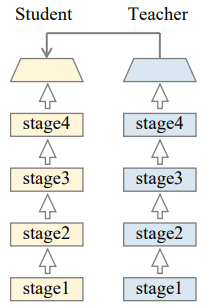
\includegraphics[scale=0.7]{19}}\end{minipage}\\
		\qquad  \qquad \qquad \qquad \qquad \qquad \qquad \qquad 知识蒸馏训练策略的整体网络结构\\
		\begin{tabular} {@{}l@{}}\noindent\textbf{2.6 创新点}\end{tabular}\\
		\qquad1.我们研究了研究不足的人体姿态模型效率问题,而现有的尝试主要集中在提高准确性性能,在部署\\时模型推断的成本很高。这是一个关键的问题,要解决扩大现有的深度姿态估计方法到实际应用。\\
		
		\qquad2. 我们提出了一种人体关键点蒸馏 (HKD) 模型训练方法,使之能够更有效地训练极小的人体姿态检\\测CNN网络。这是基于一种知识蒸馏的思想,这种思想已经成功地应用于指导物体图像分类的深度模型\\。特别地,我们推导了一个姿势知识精馏学习目标,将预先训练的较大的教师模型的潜在知识转移到微小\\的目标姿势估计模型中。\\
		
		\end{tabular}\\
		\hline
	\end{tabular}

\end{table}
\begin{table}[H]
		\centering
		\renewcommand\arraystretch{1.7}
	\begin{tabular}{|l|}
			\hline
		\begin{tabular}{@{}l@{}}
		
		\qquad3. 将目前泛化性较强的注意力模块 (PSAM) 加入进目前较为先进的人体姿态模型,提出了新型的人\\体姿态模型。与现有的偏好特定布局的通道道-空间组合相比,PSAM布局之间只有微小的度量差异。这\\表明 PSAM可能已经耗尽了其仅限通道和仅限空间分支中的表示能力。\\
		
		\qquad4.我们对于网络结构尾部模型增加了现泛化性好且轻量级的目标检测邻域的特征检测头,探究PP-\\PicoDet与检测下游任务的一体化的可能性。采用的检测头整体在所有模型尺寸上比其他模型结构实现了\\更好的速度和准确性之间的权衡,进一步提高现有的深度姿态估计方法到实际应用。
		\end{tabular}\\
		\hline
	\end{tabular}

\end{table}
\bibliography{example}
%\begin{table}
%\begin{tabular}{|c|c|c|c|}
%	\hline
%	\textbf{Model}                                                                    & \textit{\textbf{KIND}} & \textbf{Global Graph} & \textbf{Partial Graph} \\ \hline
%	\multirow{2}{*}{\textbf{XGBoost}}                                                 & \textit{Bitcoin}       & \begin{minipage}[b]{0.3\columnwidth}
%		\raisebox{-.5\height}{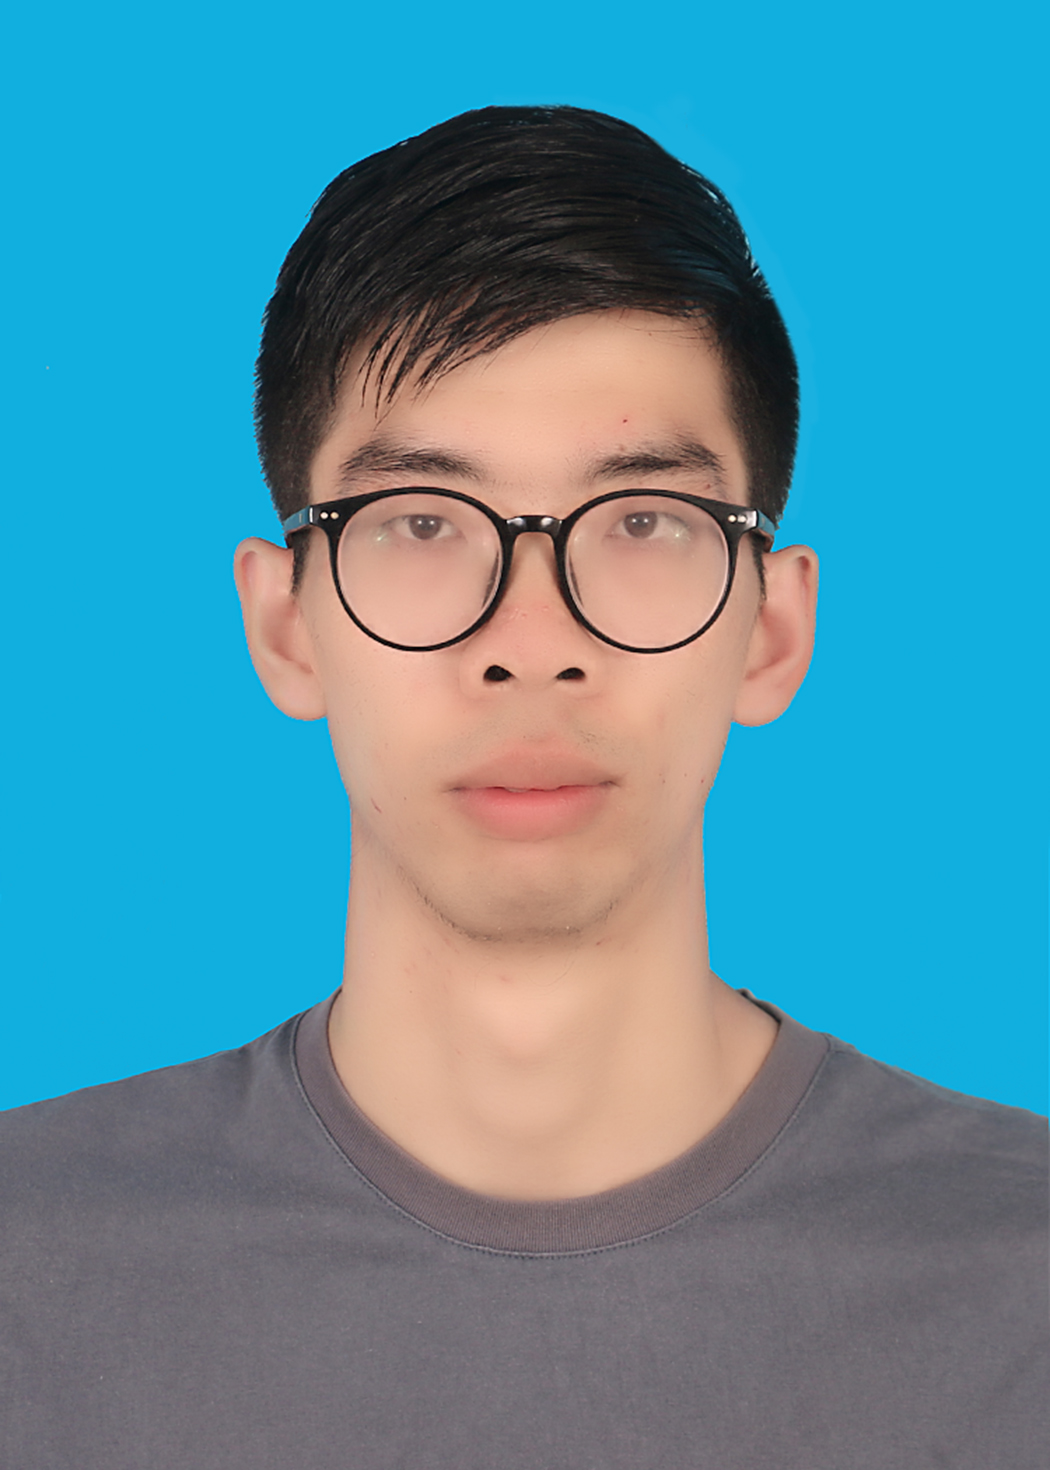
\includegraphics[width=\linewidth]{2}}
%	\end{minipage}                    &  \begin{minipage}[b]{0.3\columnwidth}
%		\raisebox{-.5\height}{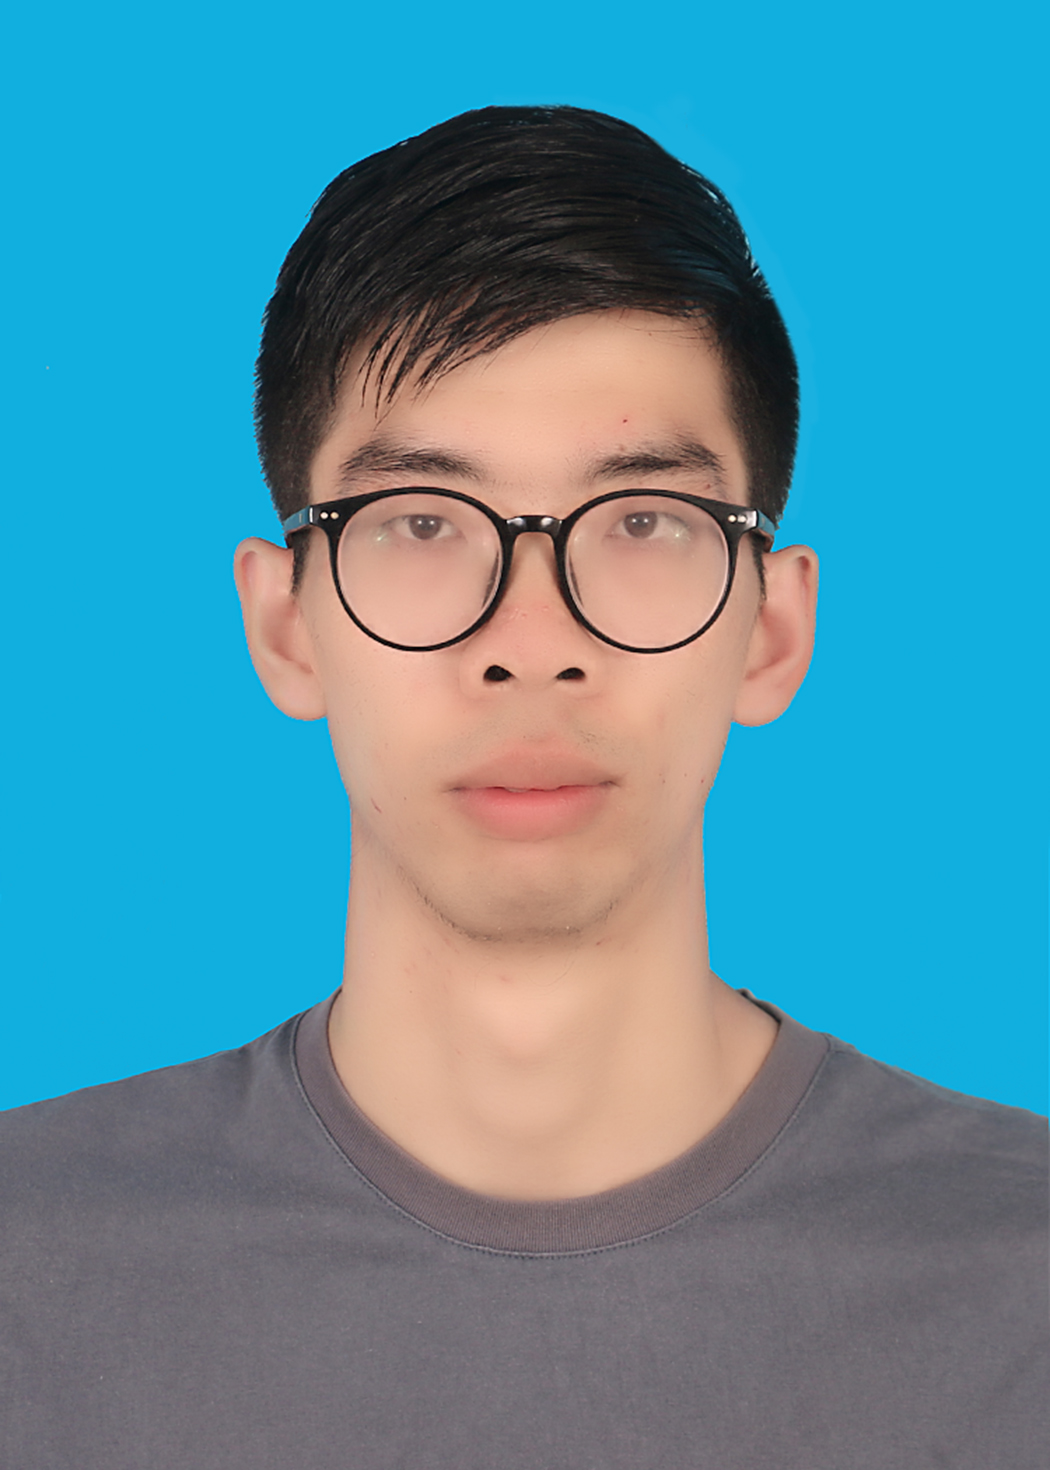
\includegraphics[width=\linewidth]{2}}
%	\end{minipage}                       \\ \cline{2-4} 
%	& \textit{Gold}          & \begin{minipage}[b]{0.3\columnwidth}
%		\raisebox{-.5\height}{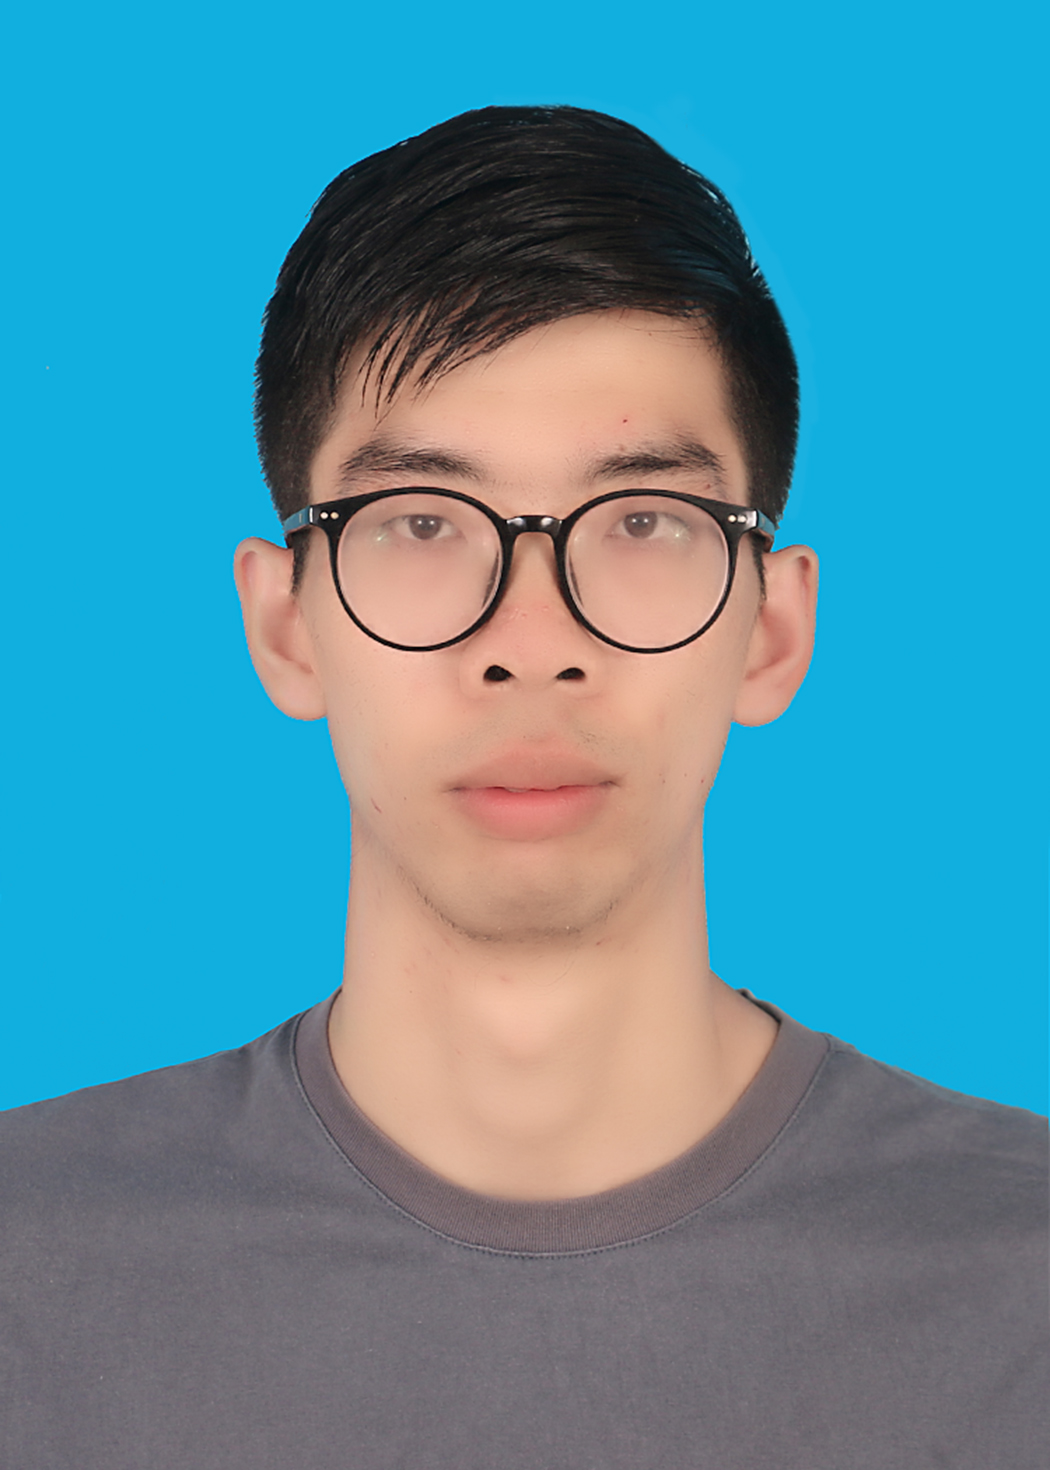
\includegraphics[width=\linewidth]{2}} 
%	\end{minipage}                    & \begin{minipage}[b]{0.3\columnwidth}
%		\raisebox{-.5\height}{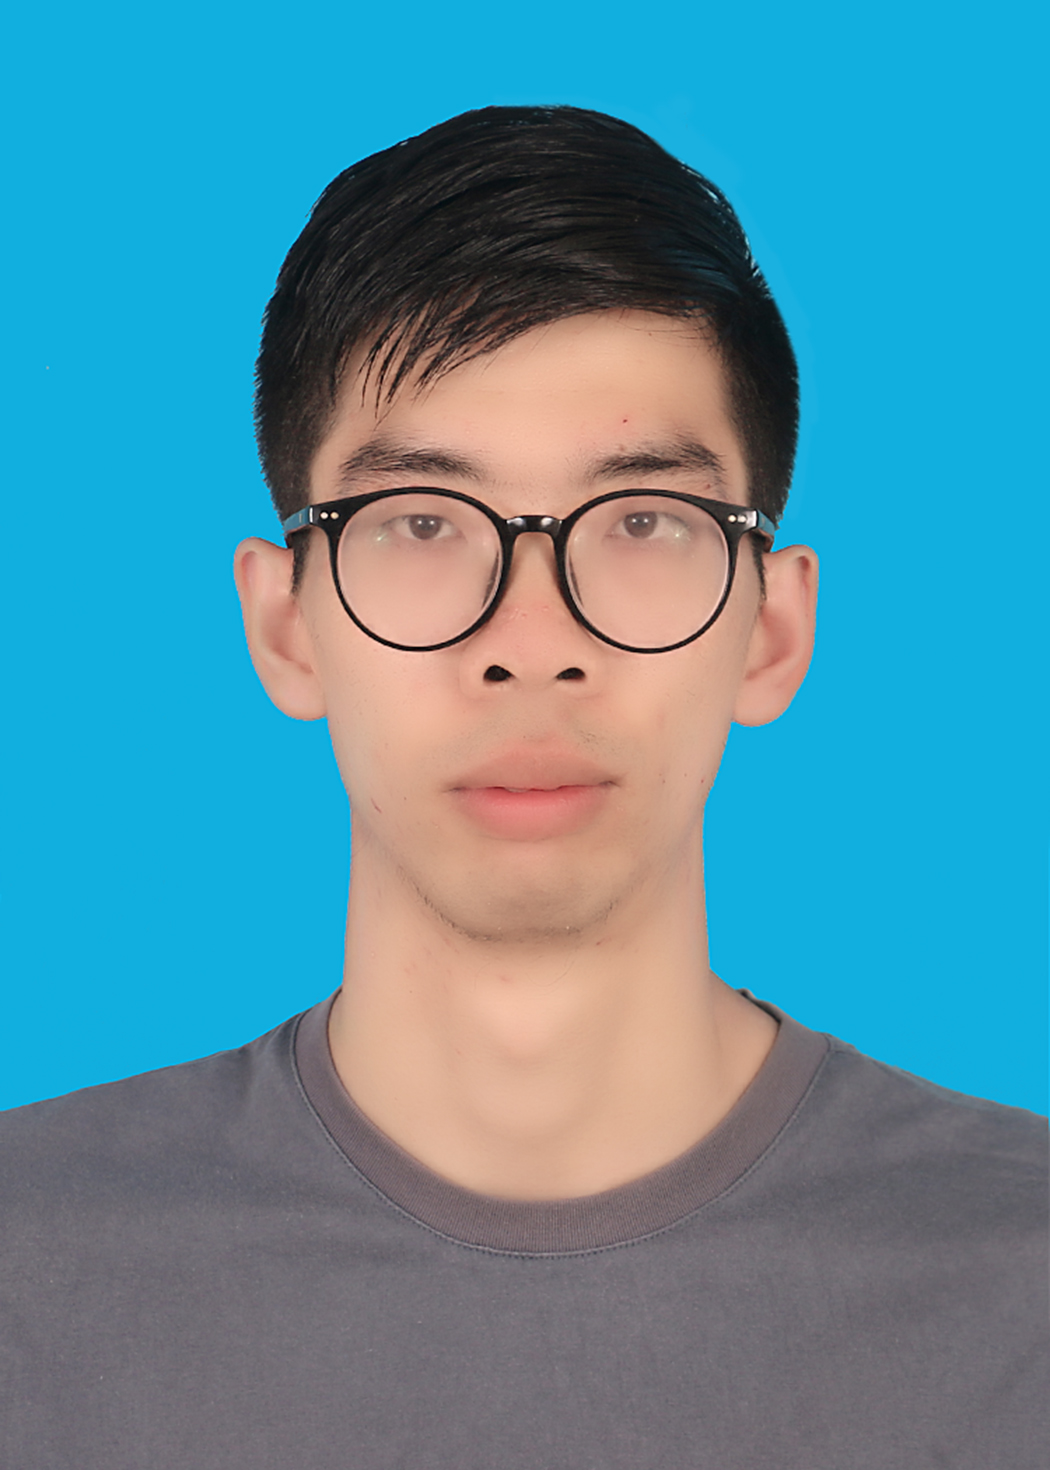
\includegraphics[width=\linewidth]{2}}  
%	\end{minipage}                    \\ \hline
%	\multirow{2}{*}{\textbf{\begin{tabular}[c]{@{}c@{}}Random\\ Forest\end{tabular}}} & \textit{Bitcoin}       & \begin{minipage}[b]{0.3\columnwidth}
%		\raisebox{-.5\height}{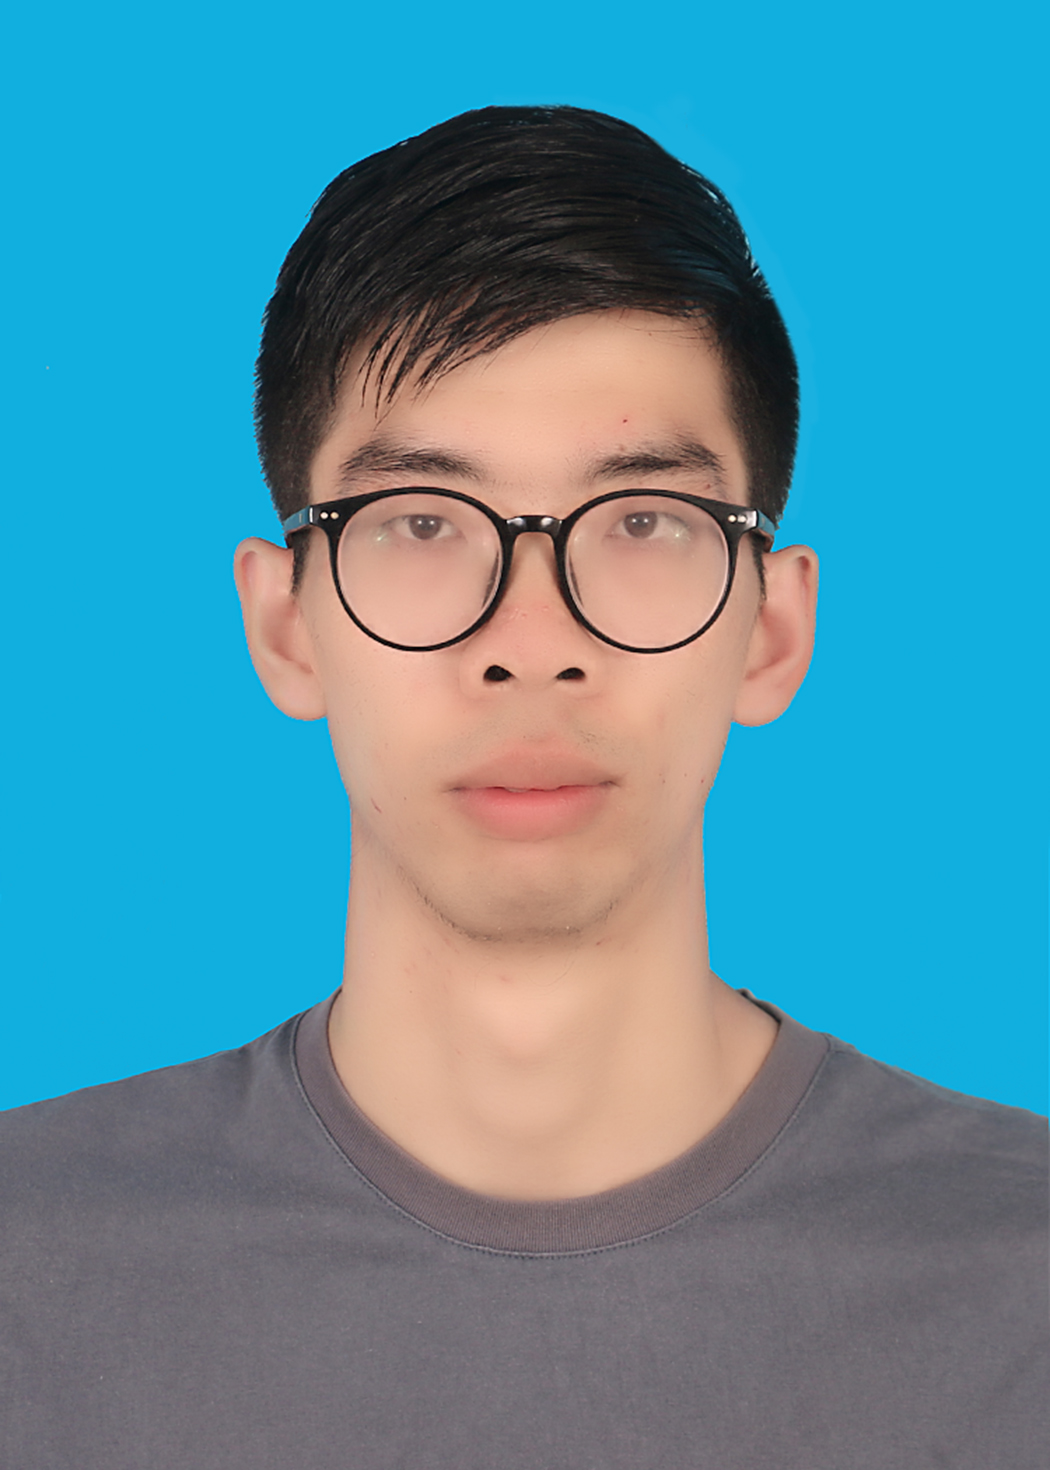
\includegraphics[width=\linewidth]{2}}
%	\end{minipage}                      & \begin{minipage}[b]{0.3\columnwidth}
%		\raisebox{-.5\height}{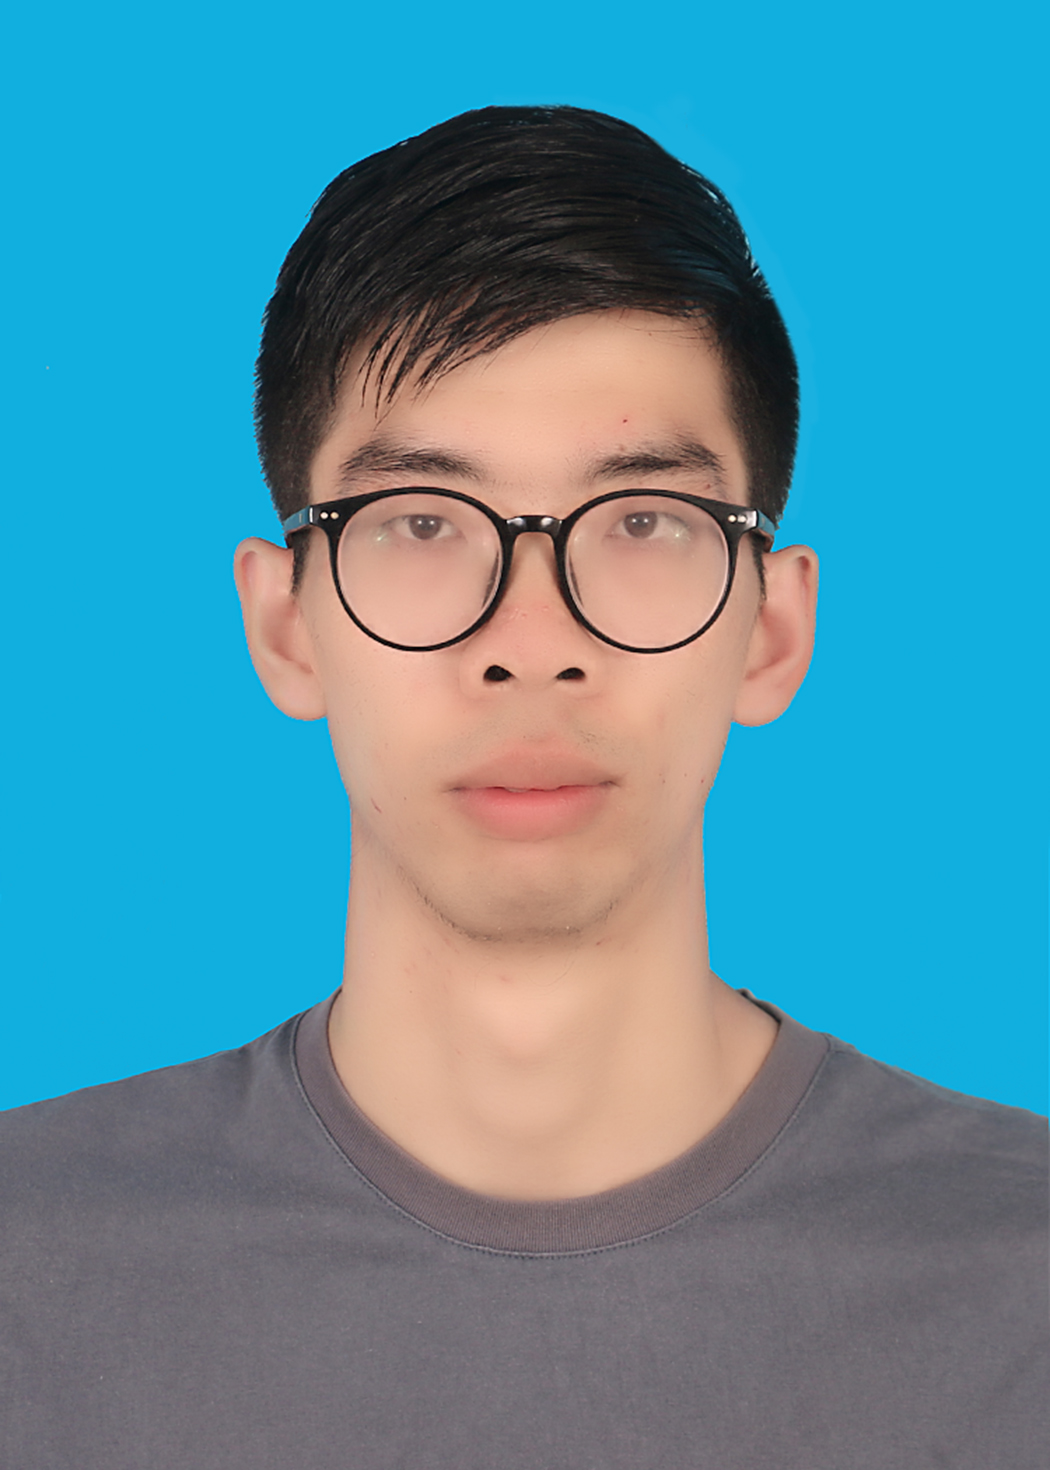
\includegraphics[width=\linewidth]{2}} 
%	\end{minipage}                       \\ \cline{2-4} 
%	& \textit{Gold}          & \begin{minipage}[b]{0.3\columnwidth}
%		\raisebox{-.5\height}{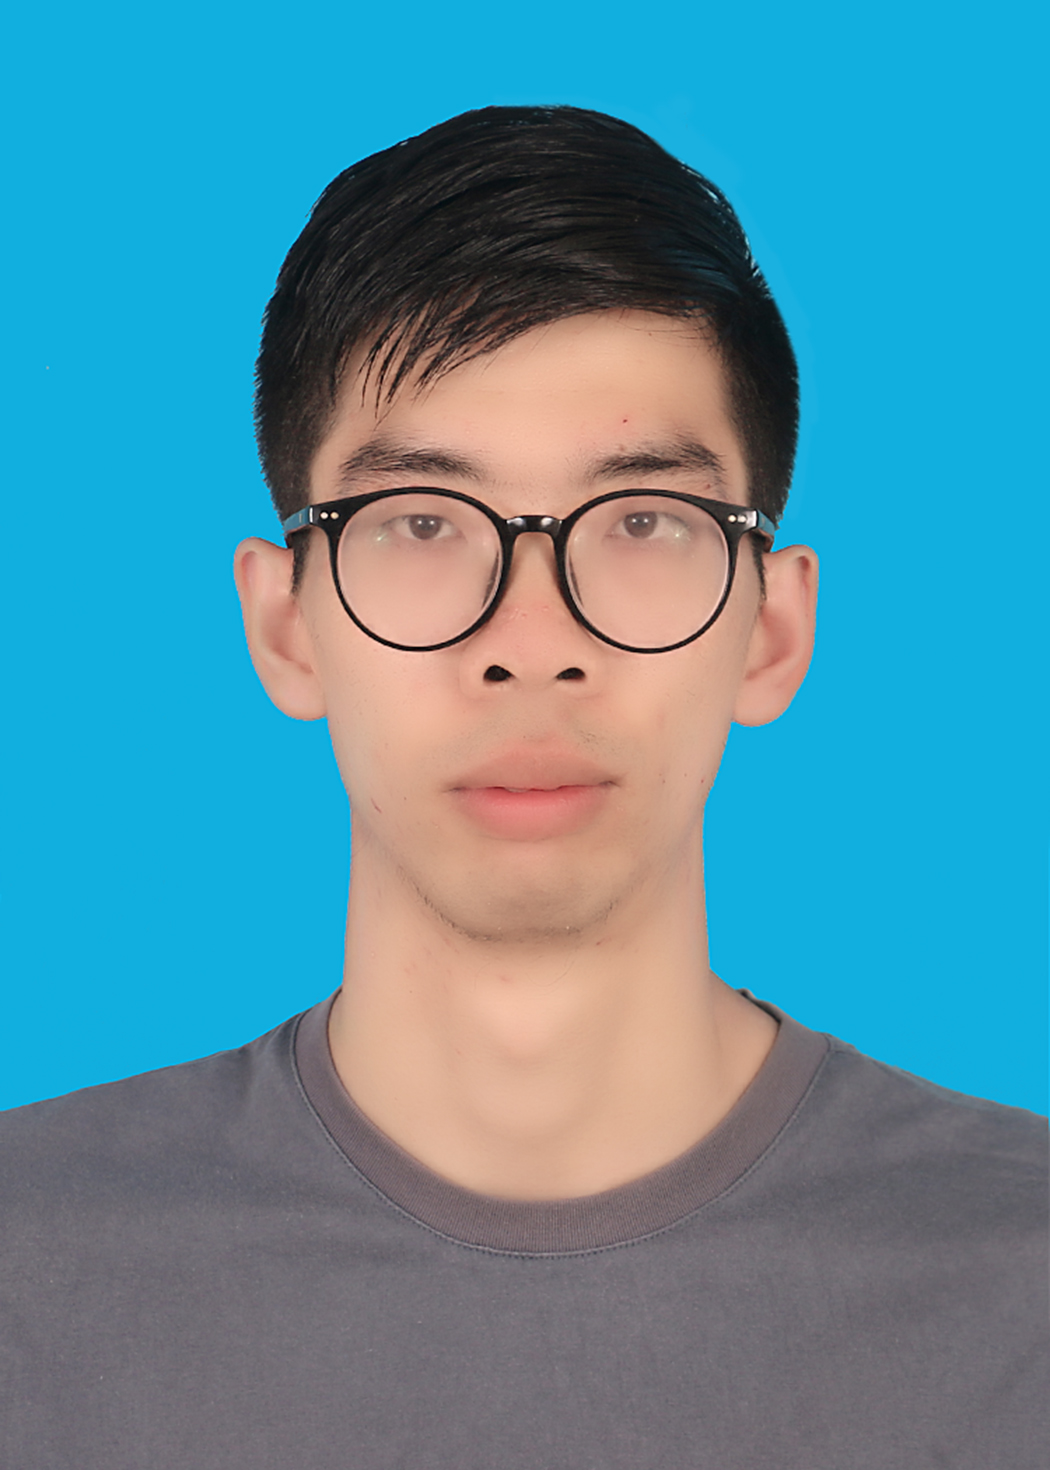
\includegraphics[width=\linewidth]{2}} 
%	\end{minipage}                      & \begin{minipage}[b]{0.3\columnwidth}
%		\raisebox{-.5\height}{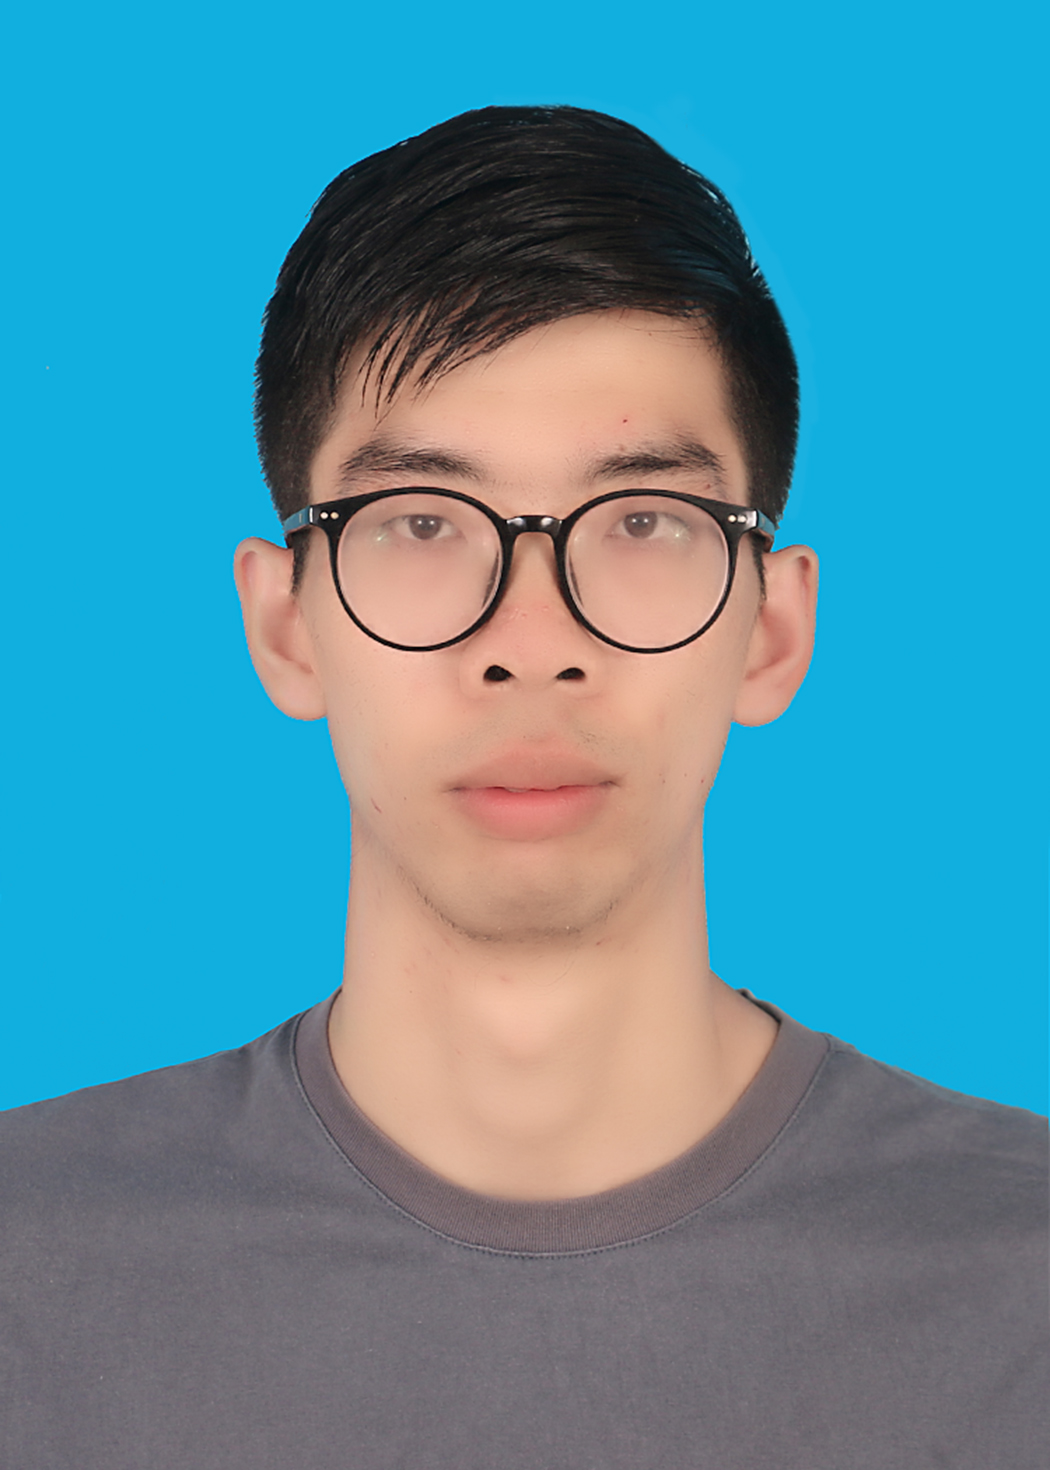
\includegraphics[width=\linewidth]{2}} 
%	\end{minipage}                       \\ \hline
%	\multirow{2}{*}{\textbf{LSTM}}                                                    & \textit{Bitcoin}       & \begin{minipage}[b]{0.3\columnwidth}
%		\raisebox{-.5\height}{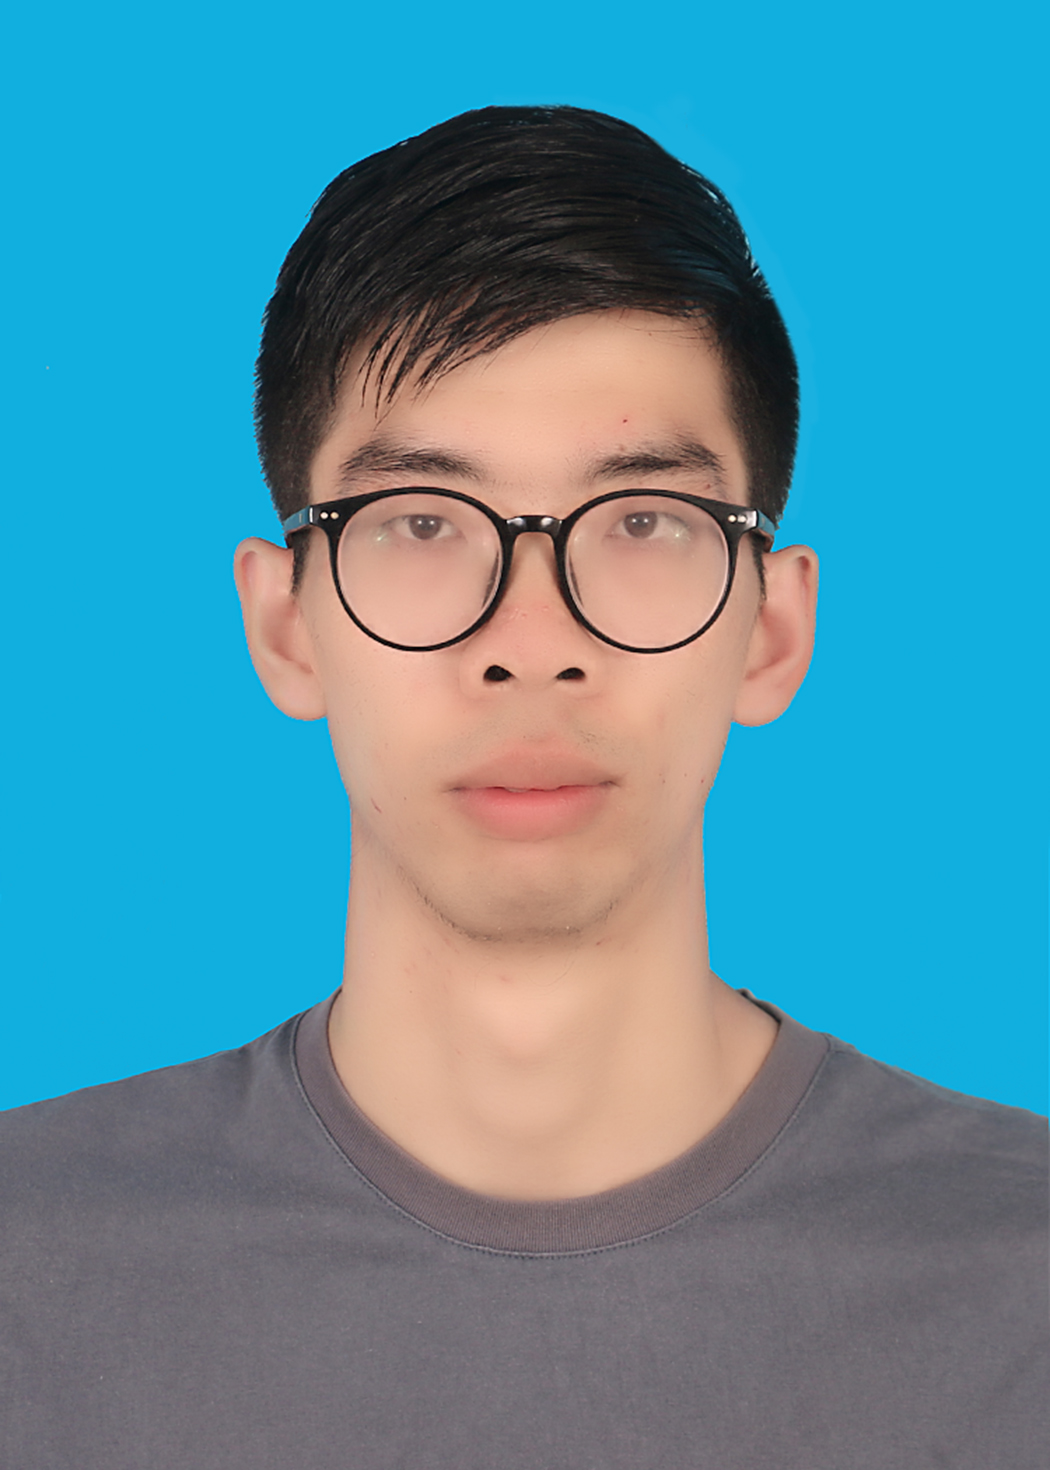
\includegraphics[width=\linewidth]{2}} 
%	\end{minipage}                      & \begin{minipage}[b]{0.3\columnwidth}
%		\raisebox{-.5\height}{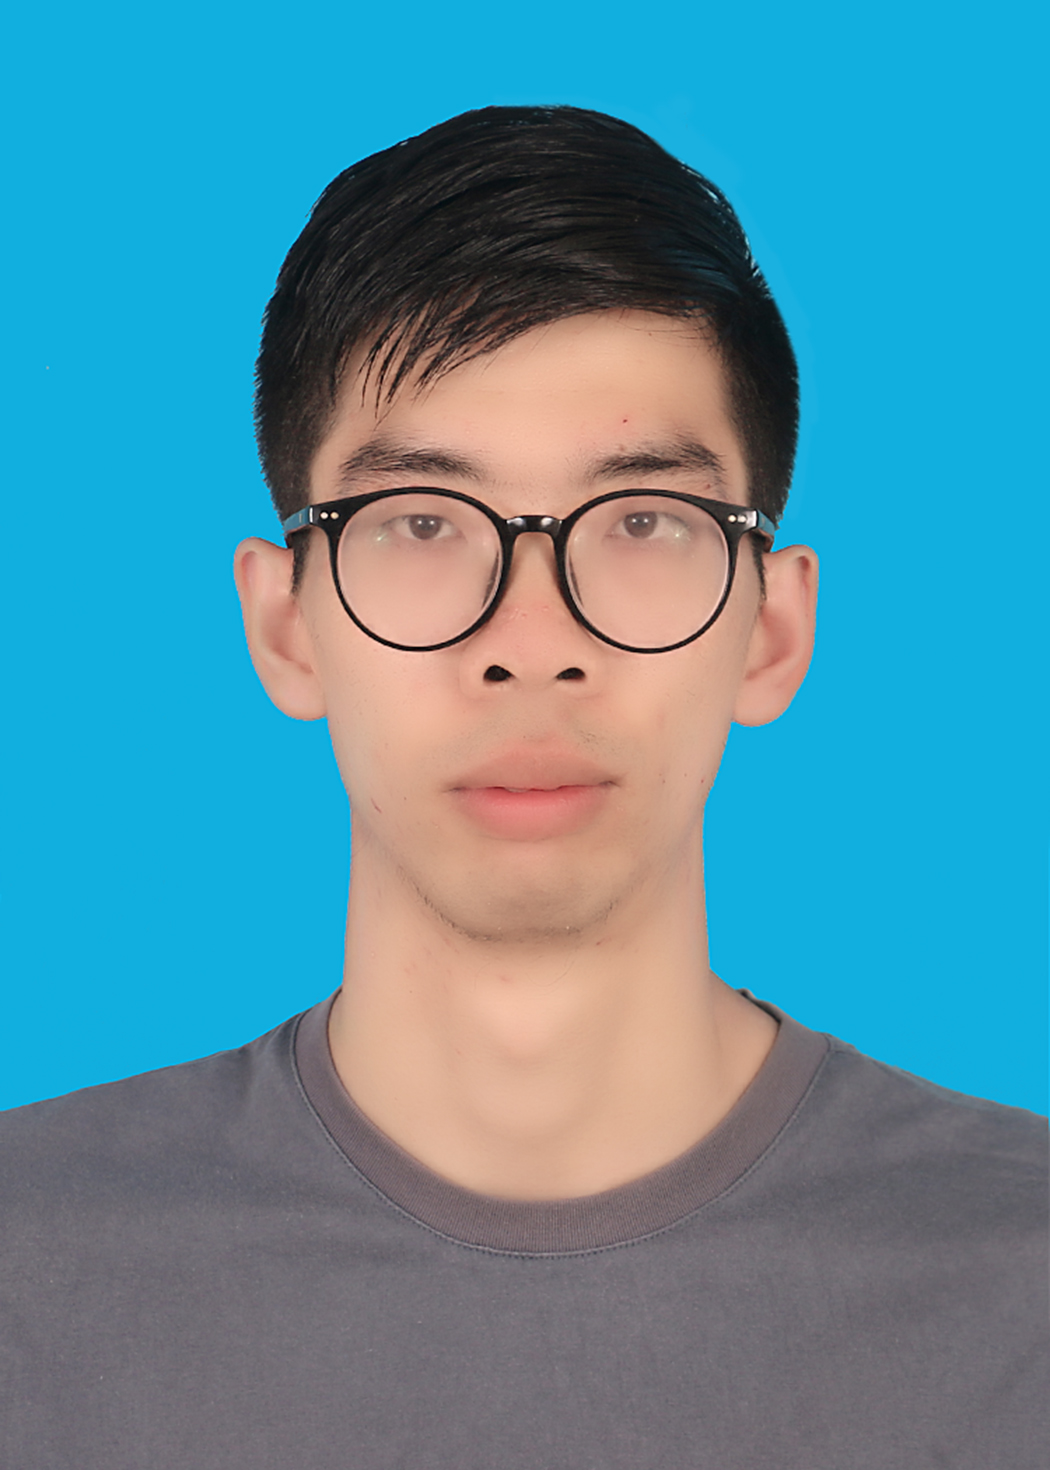
\includegraphics[width=\linewidth]{2}} 
%	\end{minipage}                       \\ \cline{2-4} 
%	& \textit{Gold}          &  \begin{minipage}[b]{0.3\columnwidth}
%		\raisebox{-.5\height}{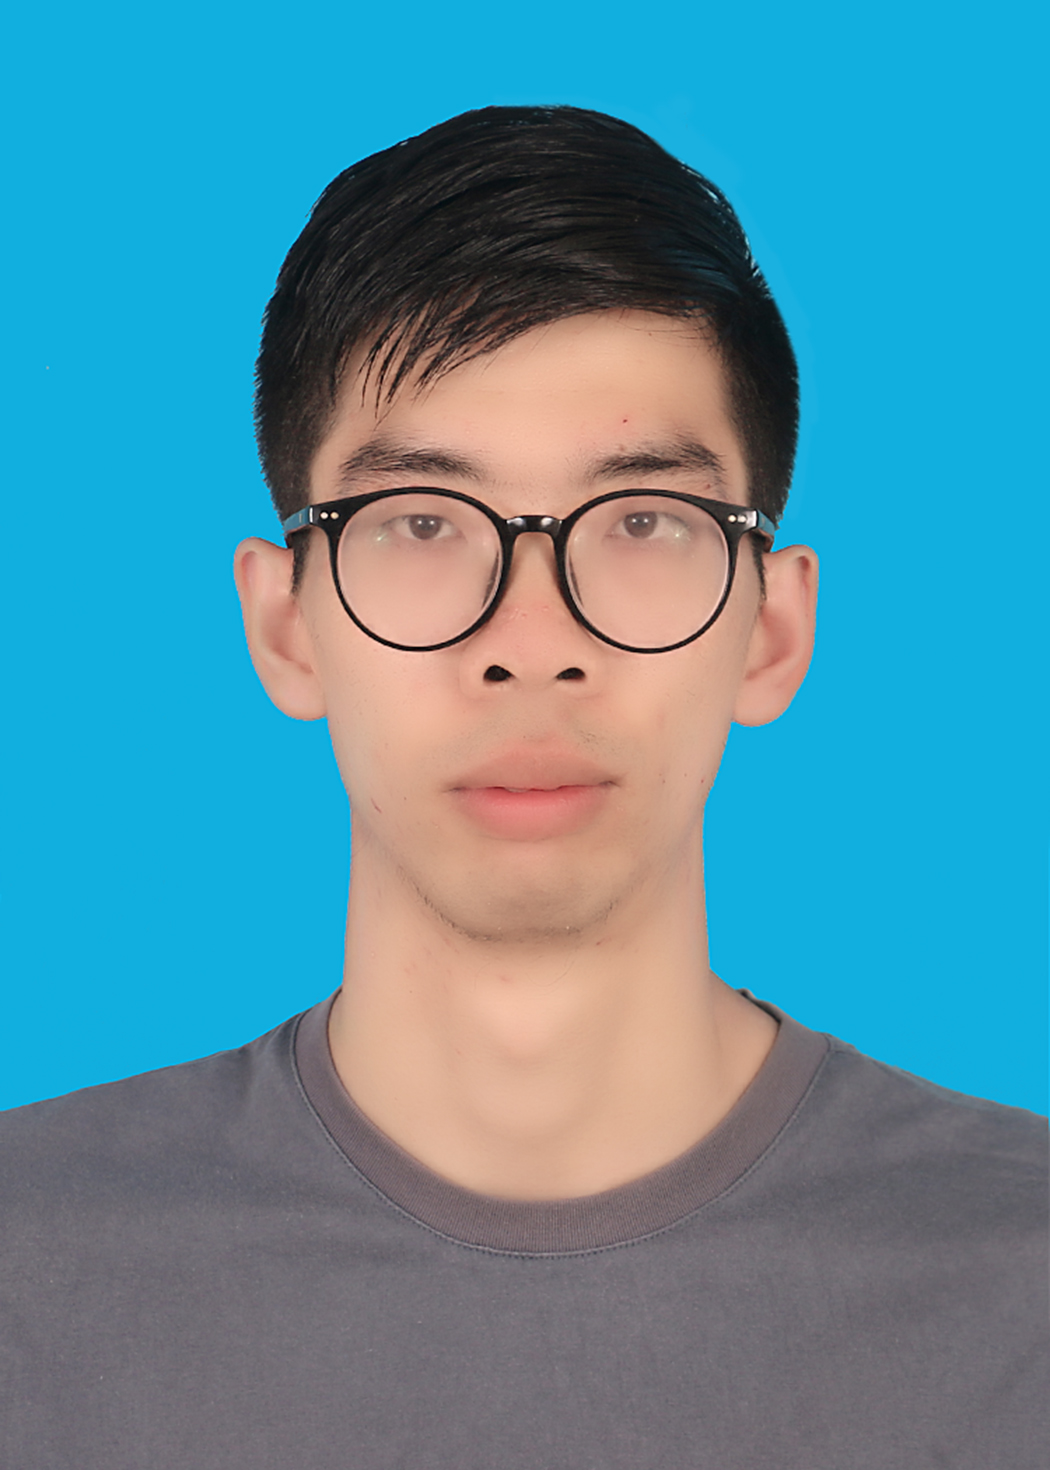
\includegraphics[width=\linewidth]{2}} 
%	\end{minipage}                     &  \begin{minipage}[b]{0.3\columnwidth}
%		\raisebox{-.5\height}{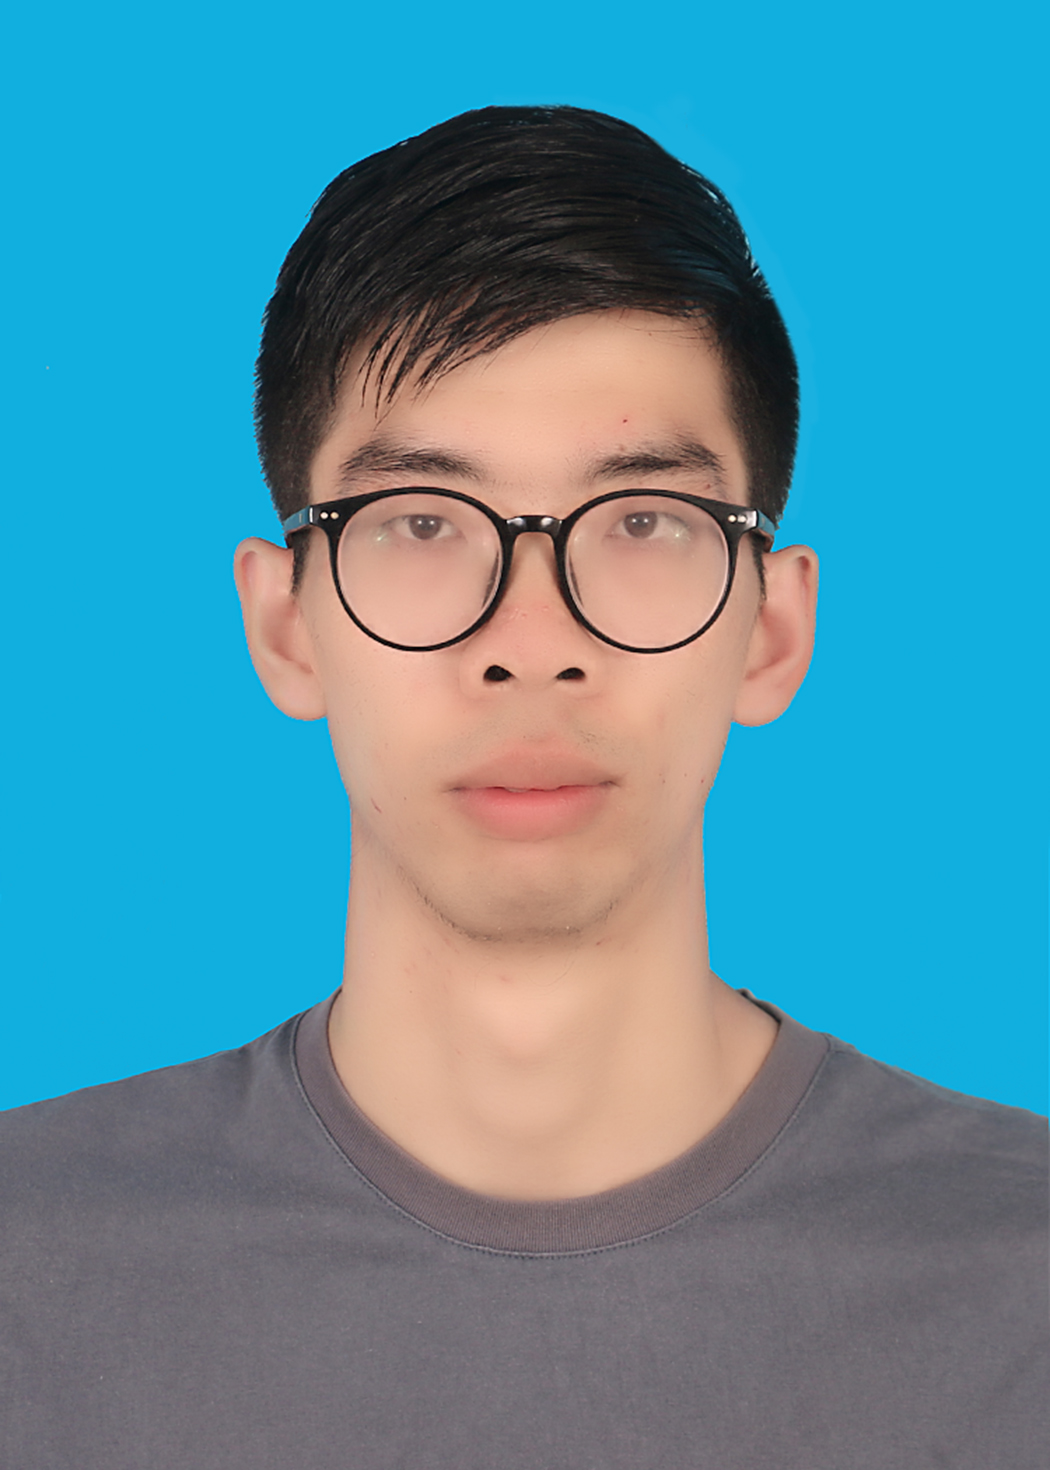
\includegraphics[width=\linewidth]{2}} 
%	\end{minipage}                      \\ \hline
%\end{tabular}
%\end{table}

%\section{学习做研究}
%\subsection{如何进入一个研究领域}
%
%进入一个领域最简单也是最有效的办法是找一本这个领域最早的论述专著或教材。当你把这个领域的基本概念的内涵以及相互之间的关系搞清楚了之后,再去读这个领域的论文,你就会因为心中有数而能够很好地把握了。这种工作必须要先做,不可以在网上乱搜论文,否则,你会感到:看了20篇文章,对这个领域的认识还没有形成,这些概念自相矛盾。由此认识还算幸运,有的人恐怕被偏见所引导,还不知道,这是最可怕的。
%
%\subsection{如何得到导师的指导}
%
%研究生期间应该开始培养独立研究的能力,所以导师一般采用宽松管理。除了几个重要的时间点老师会主动的找学生以外,其余时间都需要学生主动与老师联系。导师是否真的成为你的导师,完全要看你自己的努力,同届的几个学生,可能会得到不同数量的指导,这并不是导师厚此薄彼,而是平时交流频度和质量决定的。因此,我的建议是:
%
%1)自觉地将阶段性成果向导师汇报,听听导师的建议,老师也许会从研究方法和细化问题的角度帮助你反思,更多的时候是为你提供其它的数据来源和支持(人力、物力)。
%
%2)认真地完成老师交给你的看似与你的论文并无关系的事情。老师往往根据对你的直觉认识,认为你合适做什么事情而分配给你一些工作,也许别人对你也是这个印象,也许这是你自己都没有察觉到的你的优势。认真地有意识地发展这方面的知识和技能,会使你成为一个有特长的人。
%
%3)和老师的接触有正式和非正式两类,正式的需要预约,真的是有事情要讨教。非正式的包括路过老师的门口,打个招呼,闲聊两句。有时候正是这种无心插柳,可能带来了很多的机会和资源,也可以得到一些意想不到的指点。
%
%4)不要唯导师命是从,有时候导师分配给你某个任务也有投石问路的意思,是因为想发掘你的潜力。所以多和导师交流你的兴趣和想法,可以方便老师分配给你所想要的机会,做你想做的事情。
%
%5)记住,任何时候研究中遇到问题,都可以直接进入导师办公室,寻求帮助,即使你认为是你自己的问题。这样做的另外一个好处是,让老师知道你是因为有问题而进展停滞,而不是忙其它事情去了。
%
%\subsection{研究生期间要学什么}
%我认为研究生期间学生应该学三件事情:
%
%1)建立合理的知识结构:尽量广地涉猎学科基本知识,尽量深地了解所研究领域的方方面面、过去和现在
%
%2)掌握独立研究的方法和技能:尽量多的学习各种研究方法,熟练掌握研究过程和步骤
%
%3)学会写论文:写论文不仅是训练表达能力,更是训练思维的逻辑性,论文体例虽是八股,但却是整理思路、与他人沟通的有效结构,不可不尊重
%
%如果能够按照这三条要求自己,毕业后做不做本专业,并不重要,因为你的研究素质已经建立了,做什么事情都没有问题了。
%
%研究生不能同大学生一样学习,不能主要靠听课做笔记。如果学习的重点是听课,这样的学习就有点类似大学生的学习了。我觉得研究生就是要更多与老师对话,不能只听老师讲,而要更多地与老师讨论,要敢于主动地讲自己的学习体会。所以我希望你们能够多讲,尤其在专业课上,你们要多讲。譬如英帝国史这门课每个学期每个人可以争取主讲几个问题,如讲三个问题。我给你们列了许多小专题,提供了书目,你们可以选择一些问题来探讨。你们讲,我来听,我们互相讨论。研究生学习要有研讨气氛,要有经常性的、体制性的讨论课。讲完后,你们就每一个问题写一篇文稿,我可通过批改文稿,进一步发现你们在探讨这些问题中存在的不足和值得注意的地方。
%
%关于学习做研究的问题,这主要包括两个方面:一、培养研究素质,二、学会写论文。我先简单谈一谈培养研究素质的问题,然后再重点讲如何写论文。
%
%研究素质是什么?不同的学者可能有不同的看法。就我们这个学科而言,我认为研究素质主要包括以下因素。第一,科学态度。科学态度不是与生俱来的,必须认真培养,关键是培养我们在研究中认真负责一丝不苟的精神。第二,献身精神。从事深度学习研究,就像从事其他任何科学研究一样,要有一种为科学研究而献身的精神,要热爱我们的研究事业,要有潜心从事这项工作的意志。没有献身精神,当然做不好科研工作。只想拿一个学位,那是很难学好做研究的。要拿学位,这一点可以理解,但我们读书,是为了自己获得真才实学。有了真才实学将来不论做什么工作,都是有用的。当然学位也是要的,但关键的是学问而不是学位。第三,查阅收集学术信息、资料的能力。青年学生要从事学术研究,就要培养能熟练地掌握查阅搜集学术信息、资料的能力。例如学习与研究深度学习,就得了解国内外有关这个专业的基本情况,了解有关资料情况。像我们在赣州地区学习,至少要大致了解赣州地区有关深度学习的中英文资料,熟悉与专业密切相关的主要图书馆,了解馆藏情况。这就需要经常去图书馆。我们这个专业不需要到田间考察,到工厂调研,但要去图书馆,去图书馆就是我们的调查研究。熟悉有关图书馆的情况是我们学习的一部分。今天,网络飞速发展,掌握网上查阅信息的技巧是非常必要的。第四,处理资料的能力。搜集的资料会越来越多,怎样安排它们也是一门学问。各学科各个研究人员的方式可能会有所不同,但总的原则是要有条理,便于记忆,便于查阅。第五,对资料的鉴别意识与鉴别能力。我们在使用研究资料时不能拿着就用,要有意识鉴别一下,材料是否可靠,什么样的材料更有价值。读书时,也不是拿着什么书就通读到底。有的书翻一翻即可,有的书则需认真读。区别哪些书翻一翻即可,哪些书得认真读,也不是一件容易的事,青年学生不是一下子就能做到这一点的,需逐渐培养这种能力。还有一点就是要学会使用计算机,能比较熟练地进行文字处理。
%
%研究生学习的一项基本内容是学会写论文,如何撰写论文,我的体会是:写论文有四个基本步骤。第一,大量阅读有关著述,掌握有关资料;第二,从中发现问题,确定自己要写的论文的大致题目;第三,根据自己确定的选题,有目标地搜集能够搜集到的一切资料;第四,撰写论文本身。
%
%在写作之前,我们往往得做一件十分重要的工作,即专有名词的确定。在这一点上,对某些外文资料中的专有名词要译成中文。如何译,有时要费很大力气。还有,英文著作中的学术概念,我们要准确理解,有些概念在使用时,需赋予新的含义,不能拿来就用,要着力建立自己的概念体系和思想体系。
%
%下面我想重点谈一下撰写论文的具体过程。第一,熟悉搜集到的有关资料,对某些问题形成基本看法,再列出一个写作提纲。第二,根据写作提纲回过头来重新阅读有关资料,并运用相关资料阐述史实和自己的看法,构成一篇文稿。现在对你们来说都需要用计算机来处理文稿,这样要方便得多,尤其便于修改。第三,初稿写成后,要进行基本的文字修改。像我们的英帝国史专业,由于所引用的资料几乎全是英文,而且多半是档案文件材料,比一般著作更难读懂。在写初稿应用材料时,实际上同时在做翻译工作。在写初稿时,为了保证思路流畅,对于翻译文字不能仔细推敲,所以初稿写成后,文字很粗糙。那么在修改时,一项基本任务就是反复推敲原文材料,看自己的理解和中文表达是否准确,是否符合原文。在写初稿时要简要注明材料的出处,便于修改时查对,即使有些地方在正式发表时不一定需要做注释,但在初稿时却要标明,以便自己修改和查对。这样进行文字修改后,形成第二稿,打印出来。
%
%在第二稿的基础上,还需认真进行一次文字修改。修改文字时,一个非常重要的任务是,避免文字的洋味。我们使用的是英文材料,由于英文和中文在语法结构上有很大区别,文字表达上也很不相同,在运用材料时,往往容易出现带有洋味的中文。这是我写作过程中容易犯的毛病,也是青年学生容易犯的通病。我们要尽量用标准的中文写作。在用英文材料时,我更强调的是准确,而不是文字的优美。当然,文字要尽可能优美,但不能以牺牲准确为代价。在第二稿时,一般要认真做注释,按通常的学术标准做注释。做注释也是一门学问,必须认真对待,好好学习,不能采取无所谓的态度,这涉及到是否采取科学态度的问题。注释做好了,便于自己和读者查阅。在做注释上,有两点我想特别提出来,一是引用别人的观点,不管是正式发表的还是尚未正式发表的,都要注明。二是自己从哪里看到的材料,就注明从哪里引用的,不能弄虚作假。例如,有些档案材料,自己并没有亲眼看过,而是从别的作者的著述中看到的,就不能像自己亲自看了一样作注,应写明转引自或直接注明引自某著述。做了注释,这样可以形成第三稿。
%
%第三稿打印出来后,进一步进行文字修改,把所有表达不清的地方说清楚,把所有赘句、赘词、赘字全都删掉,使文字向简洁优美靠拢,思路清晰,逻辑严密。当然,文字功夫的提高是没有止境的。要不断学习。冰冻三尺,非一日之寒。所以第三稿还要回过头来认真查对每个注释是否有误,是否有不符合标准的地方。对于人名、地名、时间等,没有百分之百的把握时,就得查对。
%
%经过这样修改之后,文章已基本定型。此时,我的经验是打印一稿,放一段时间,然后再最后定稿。定稿时有两大任务:一、进一步进行文字润色,尽量做到简明易懂:二、如感到对某些史料不踏实,还要进行查对,直到每一处都准确可靠为止。下一步才能把文稿付诸发表。
%\section{人体姿态识别综述}
%\subsection{单人姿态估计}
%2015 年之前的方法都是回归出精确的关节点坐标( x,y ),采用这种方法不好的原因是人体运动灵活,模型可扩展性较差。本文主要是2015年之后人体姿态识别的发展综述。(1)遮挡问题,这个问题恐怕是最难的,也是必须要解决的(2)速度过慢。(3)仅仅有二位的姿态是不够的,目前也有这一类的研究,关于直接从2d到3d的姿态进行直接估计。这一点是未来发展的趋势。
%
%单人姿态估计性能评价指标:MPII单人数据集,LSP数据集和FLIC数据集。通过对比这三个数据集的PCK值来评价模型好坏。评价指标为PCK(Percentage of Correct Keypoints)即关键点正确估计的比例,计算检测的关键点与其对应的groundtruth 间的归一化距离小于设定阈值的比例,FLIC中是以躯干直径作为归一化参考,MPII中是以头部长度作为归一化参考,即PCKh。
%
%\textbf{发展历程:}
%
%1.《Flowing ConvNets for Human Pose Estimation in Videos》ICCV 2015
%
%2015 年 flow convnet 将姿态估计看作是检测问题,输出是 heatmap。用相对于AlexNet更深的CNN网络进行人体姿态估计,提高关节点定位的鲁棒性,利用temporal提高精度。其创新点在于从卷积神经网络的 3 和 7 层提取出来,再经过卷积操作,称之为空间融合模型,用来提取关节点之间的内在联系;同时使用光流信息,用来对准相邻帧的 heatmap 预测。最后使用参数池化层,将对齐的heatmap 合并成一个 scoremap(置信图)。
%
%网络pipeline:对于当前帧t,输入它的相邻的前后n帧。利用全卷积神经网络(Spatial Net + Spatial Fusion Layers)对每一帧输出一个预测的heatmap。再利用光流信息将这些heatmap扭曲到当前帧t。之后将warped的heatmap合并到另一个卷积层中,该层学习如何权衡来自附近框架的扭曲的heatmap。最后使用集合热图的最大值作为人体的身体关节。
%
%评测数据集:FLIC数据集,对于wrist(手腕)和elbow(肘部)的平均PCK可以达到92\%,可以做到实时性,速度为5fps。但是该方法对于pose的估计范围有限,只是半身的关节点,并不是全身的身体骨骼点。
%
%2.《Convolutional Pose Machines》CVPR 2016
%
%2016 年提出的 CPM 方法具有很强的鲁棒性,之后的很多方法是基于此改进的。CPM 的贡献在于使用顺序化的卷积架构来表达空间信息和纹理信息。网络分为多个阶段,每一个阶段都有监督训练的部分。前面的阶段使用原始图片作为输入,后面阶段使用之前阶段的特征图作为输入,主要是为了融合空间信息,纹理信息和中心约束。另外,对同一个卷积架构同时使用多个尺度处理输入的特征和响应,既能保证精度,又考虑了各部件之间的远近距离关系。
%
%网络输入彩色图像(绿色ori image)。以半身模型为例,分为四个阶段(stage)。每个阶段都能输出各个部件的响应图(蓝色score),使用时以最后一个阶段的响应图输出为准。center map(绿色)是一个提前生成的高斯函数模板,用来把响应归拢到图像中心。 第一阶段是一个基本的卷积网络1(白色convs),从彩色图像直接预测每个部件的响应。半身模型有9个部件,另外包含一个背景响应,共10层响应图。第二阶段也是从彩色图像预测各部件响应,但是在卷积层中段多了一个串联层(红色concat),把以下三个数据合一:
%
%阶段性的卷积结果为46*46*32纹理特征 , 前一阶段各部件响应为46*46*10 空间特征 ,中心约束(46*46*1) ,串联后的结果尺寸不变,深度变为32+10+1 = 43。第三阶段不再使用原始图像为输入,而是从第二阶段的中途取出一个深度为128的特征图(feature image)作为输入。同样使用串联层综合三种因素:纹理特征+空间特征+中心约束。 第四阶段结构和第三阶段完全相同。在设计更复杂的网络时(例如全身模型),只需调整部件数量(从10变为15),并重复第三阶段结构即可。
%
%该论文的主要训练细节有三:1. 数据增强:对原始图片进行随机缩放,旋转,镜像2. 标定:在每个关节点的位置放置一个高斯响应,来构造响应图的真值。对于含有多个人的图像,生成两种真值响应,一是在每个人的相应关节位置,放置高斯响应。二是只在标定的人的相应关节位置,放置高斯响应。3. 中继监督,多个loss:如果直接对整个网络进行梯度下降,则输出层在经过多层反向传播会大幅度的减小,解决方法就是在每个阶段都输出一个loss,可保证底层参数正常更新。
%
%评测数据集:MPII,LSP,FLIC,在MPII数据集上的total PCKh是87.95\%(如果加上LSP数据集作为训练,将达到88.52\%),在LSP数据集上的PCKh是84.32\%(如果加上MPII数据集作为训练,将达到90.5\%),在FLIC数据集上的PCK@0.2分别是elbows(97.59\%),wrist(95.03\%)。
%
%3.《Stacked Hourglass Networks for Human Pose Estimation》ECCV 2016
%
%本文使用全卷积网络解决人体姿态分析问题,截至2016年5月,在MPII姿态分析竞赛中暂列榜首,PCKh(误差小于一半头高的样本比例)达到89.4\%。与排名第二的CPM(Convolutiona Pose Machine)1方法相比,思路更明晰,网络更简洁。该论文体现了从模块到网络再到完整网络的设计思想。
%
%使用的初级模块称为Residual Module,得名于其中的旁路相加结构。Residual模块提取了较高层次的特征(卷积路),同时保留了原有层次的信息(跳级路)。不改变数据尺寸,只改变数据深度。可以把它看做一个保尺寸的高级“卷积”层。
%
%4.《Adversarial PoseNet: A Structure-aware Convolutional Network for Human Pose Estimation》ICCV 2017
%
%采用的GAN的方法,效果比之前的state-of-the-art仅仅提升了零点几个百分点。基本上到hourglass之后的方法都是一些微调,虽然理论都不太一样,但是准确度提升不大。
%
%5.《Learning Feature Pyramids for Human Pose Estimation》ICCV 2017
%
%模式识别的方法,pictorial structures以及loopy 结构,这些方法都是基于HOG 特征。后来是神经网络,最早的是deepPose,是使用回归坐标点的方法。坐标点难以训练学习,后来的方法都是将点做了高斯转换得到score map。同时,还会用到多尺度获得丰富特征。
%
%多尺度特征Hourglass无疑是最成功的。但后面的多种网络结构对这这一基础网络做了调整和优化,有更好的效果。比如这篇,将使用金字塔模型。不是普通的金字塔,而是组合了residual模型和Inception的金字塔,所以计算要求不高。
%\subsection{多人姿态估计}
%1.《DeepCut: Joint Subset Partition and Labeling for Multi Person Pose Estimation》 CVPR 2016
%
%2016 年的 deepcut,采用自顶向下的方法,先用 CNN 找出所有候选的关节点,将这些关节点组成一幅图,对图中的节点进行聚类,从而判断各个节点属于哪一个人,这是一个优化问题;同时,对各个点进行标记,分类属于身体的哪一部分;两者结合输出姿态估计结果。
%
%Deepercut 是在 deepcut 的基础上使用 resnet 进行检测提高精度,使用 image conditioned pairwise ,能够将丰富的候选节点进行压缩,提升速度和鲁棒性。
%
%评测数据集:deepcut,对于单人姿态估计,在LSP数据集上的PCK达到87.1\%,在MPII数据集上的PCK达到82.4\%(可见,适用于多人的姿态估计方法和纯粹的单人姿态估计方法的准确率还有所差距);对于多人姿态估计,在WAF数据集上mean PCP达到84.7\%,在MPII多人数据集上AP 达到 60.5\%,速度非常慢。
%
%DeeperCut:和deepcut的评测数据集相同,这里主要针对多人来看,其准确率和速度都有所提升,尤其是速度方面。
%
%2.《ArtTrack: Articulated Multi-person Tracking in the Wild》CVPR 2017
%
%2017年的ArtTrack的作者也是DeeperCut 的第一作者,是将人物姿态估计用到了视频跟踪里面,本文的贡献是利用现有的单帧姿态估计模型作为基础框架,但是速度却明显加快,这种加快主要通过以下两种方式来进行:(1)通过简化和稀疏身体部位的关系图,使用进来的方法进行快速的推理;(2)不加载用于前馈神经网络上的大规模计算量,这些神经网络是为了检测和关联同一人的身体关节。模型仍然是采用 top-down 的方法,即先用 Resnet 检测出body part proposal,然后再根据关联和空间信息将他们归为不同的人。
%
%同时,本文也提出一种 top-down/bottom-up 的模型,即 top-down 部分是用来对人体做一个粗略的估计,之后再用bottom-up 进行精确调整,使得预测的关节点位置更准确。
%
%评测数据集:WAF数据集和MPII Video Pose数据集,相应有所提升。
%
%3.《Realtime Multi-Person 2D Pose Estimation using Part Affinity Fields》CVPR 2017
%
%2017 年的 Part Affinity Fields(PAF)能够针对多人做到实时检测,它采用的却是自底向上的方法,网络框架分为两路;一路使用 CNN,根据置信图进行关节点预测,另一路使用CNN 获得每个关节点的 PAF,PAF 可以看作是记录 limb 位置和方向的 2D 向量。两路进行联合学习和预测。最后就是如何将这些节点两两连接不重复,这转换为图论问题。
%
%评测数据集:COCO 2016关键点检测数据集+MPII multi-person benchmark。对于MPII多人pose,本文无论是准确度还是精度上都有质的飞跃,其相比于DeeperCut的速度快了4万多倍,准确度也有几个百分点的提升。可以做到实时,每帧只需要50毫秒,即20FPS。
%
%4.《Mask R-CNN》ICCV 2017,FAIR,Kaiming He
%
%2017年何凯明的Mask R-CNN,Mask R-CNN 是用于目标检测分割的框架,即对一张图片,既输出图片中已有的目标,还能为每一个实例生成一个高质量的分割掩码。mask RCNN是在 faster R-CNN 的基础上,在每一个 RoI 都增加一个预测分割的mask,这和分类以及 bounding box 回归是并行的一条分支。它的训练简单,仅仅比 faster RCNN多一点计算开销。它易于泛化到多个任务上,例如人体姿态估计。在不加任何的 trick的情况下,在COCO 数据集上超越其他的方法。因此准确度方面基本上已经是state-of-the-Art。
%
%应用到pose estimation,将分割系统中的目标改为K个one-hot,m*m的二进制mask。准确率比COCO 2016 冠军高0.9个点,速度达到5 FPS。
%
%5.《Towards accurate multi-person pose estimation in the wild》CVPR 2017
%
%Google的人体姿态估计,多数时候在论文中简写为G-RMI。
%
%论文采用top-down的结构,分为两个阶段: 第一阶段使用faster rcnn做detection,检测出图片中的多个人,并对bounding box进行image crop; 第二阶段采用fully convolutional resnet对每一个bonding box中的人物预测dense heatmap和offset; 最后通过heatmap和offset的融合得到关键点的精确定位。
%
%6.《Associative Embedding:End-to-End Learning for Joint Detection and Grouping》
%
%论文提出了一种single-stage,end-to-end的关节点检测和分组方法,这不同于以往的multi-stage的关节点检测方法,在MPII和COCO数据集上达到新的state-of-the-art的效果,超越最近的Mask RCNN和Google GMI。从人体姿态估计方法上属于bottom-up的方法,即先检测关节点,再对关节点进行分组。在COCO测试集上mAP达到0.655。
%
%7.《RMPE: Regional Multi-Person Pose Estimation》ICCV 2017,SJTU,Tencent Youtu
%
%文章的写作背景是单人姿态估计的方法不能用在多人上面,而多人姿态估计方法虽然效果不错,但是太慢了(485 seconds per image)。它对于多人姿态估计的方法采用传统的自顶向下的方法,即先检测人,再识别人体姿态。检测使用的是SSD-512,识别人体姿态使用的是state-of-the-art的Stacked Hourglass方法。致力于解决对于imperfect proposal,通过调整,使得crop的单人能够被单人姿态估计方法很好的识别,从而克服检测带来的定位误差。
%
%目前的人体检测方法会产生两个主要问题:定位错误,以及多余的检测结果,尤其是SPPE (singal person pose estimation)。这篇文章就是为解决这个问题而来的,提出了RMPE方法。包括了三个模块:Symmetric Spatial Transformer Network (SSTN)用于在不准确的bounding box下仍能提取准确的单个人的范围,这是组合到SPPE里面的。NMS是处理多余的候选框的,它是采用了新的距离量测的方法来计算姿态的相似度,且是数据驱动的,不是预先设定的。PGPG用于增多训练样本。
%
%\subsection{相关数据集}
%1.LSP(Leeds Sports Pose Dataset)
%
%地址:http://sam.johnson.io/research/lsp.html
%
%样本数:2K
%
%关节点个数:14
%
%全身,单人
%
%2.FLIC(Frames Labeled In Cinema)
%
%地址:https://bensapp.github.io/flic-dataset.html
%
%样本数:2W
%
%关节点个数:9
%
%全身,单人
%
%3.MPII(Max Planck institut informatik)
%
%地址:http://human-pose.mpi-inf.mpg.de/
%
%样本数:25K
%
%关节点个数:16
%
%全身,单人/多人,40K people,410 human activities
%
%4.MSCOCO(Common Objects in Context)
%
%地址:$\texttt{http://cocodataset.org/\#download}$
%
%样本数:>= 30W
%
%关节点个数:18
%
%全身,多人,keypoints on 10W people
%
%5.AI Challenge
%
%地址:https://challenger.ai/competition/keypoint/subject
%
%样本数:21W Training, 3W Validation, 3W Testing
%
%关节点个数:14
%
%全身,多人,38W people
%
%6.3D数据集:
%
%在数据处理阶段,3D比2D复杂很多。2D人体姿态识别在dataset和model方面都比3D成熟,2Dmodel也有很多户外,自然界的dataset,但是3D的dataset几乎都是indoor的。因为3D标注、识别的复杂,所以需要大量的传感器,摄像头去采集数据。收集了几个最近看到的数据集分享给大家。
%
%7.Human3.6M数据集   
%
% Human3.6M数据集有360万个3D人体姿势和相应的图像,共有11个实验者(6男5女,论文一般选取1,5,6,7,8作为train,9,11作为test),共有17个动作场景,诸如讨论、吃饭、运动、问候等动作。该数据由4个数字摄像机,1个时间传感器,10个运动摄像机捕获。
% 
%8.CMU Panoptic dataset
%
%该数据集是CMU大学制作,由480个VGA摄像头,30+HD摄像头和10个Kinnect传感器采集。
%
%9.MPI-INF-3DHP        
%
%该数据集由Max Planck Institute for Informatics制作,详情可见Monocular 3D Human Pose Estimation In The Wild Using Improved CNN Supervision论文。
\end{document}